%% 
%% Copyright 2007, 2008, 2009 Elsevier Ltd
%% 
%% This file is part of the 'Elsarticle Bundle'.
%% ---------------------------------------------
%% 
%% It may be distributed under the conditions of the LaTeX Project Public
%% License, either version 1.2 of this license or (at your option) any
%% later version.  The latest version of this license is in
%%    http://www.latex-project.org/lppl.txt
%% and version 1.2 or later is part of all distributions of LaTeX
%% version 1999/12/01 or later.
%% 
%% The list of all files belonging to the 'Elsarticle Bundle' is
%% given in the file `manifest.txt'.
%% 

%% Template article for Elsevier's document class `elsarticle'
%% with numbered style bibliographic references
%% SP 2008/03/01

\documentclass[preprint,12pt]{elsarticle}

%% Use the option review to obtain double line spacing
%% \documentclass[authoryear,preprint,review,12pt]{elsarticle}

%% Use the options 1p,twocolumn; 3p; 3p,twocolumn; 5p; or 5p,twocolumn
%% for a journal layout:
%% \documentclass[final,1p,times]{elsarticle}
%% \documentclass[final,1p,times,twocolumn]{elsarticle}
%% \documentclass[final,3p,times]{elsarticle}
%% \documentclass[final,3p,times,twocolumn]{elsarticle}
%% \documentclass[final,5p,times]{elsarticle}
%% \documentclass[final,5p,times,twocolumn]{elsarticle}

%% For including figures, graphicx.sty has been loaded in
%% elsarticle.cls. If you prefer to use the old commands
%% please give \usepackage{epsfig}

%% The amssymb package provides various useful mathematical symbols
\usepackage{amssymb}
%% The amsthm package provides extended theorem environments
%% \usepackage{amsthm}

%% The lineno packages adds line numbers. Start line numbering with
%% \begin{linenumbers}, end it with \end{linenumbers}. Or switch it on
%% for the whole article with \linenumbers.
%% \usepackage{lineno}

\usepackage{algorithm}
\usepackage{algorithmic}
%\usepackage[breaklinks]{hyperref}
\usepackage{breakcites}
\usepackage{amsmath}
%\usepackage{url}
%\usepackage{breakurl}
\usepackage[hyphens]{url}
\usepackage{hyperref}

\journal{Journal of Systems and Software}

\begin{document}

\begin{frontmatter}

%% Title, authors and addresses

%% use the tnoteref command within \title for footnotes;
%% use the tnotetext command for theassociated footnote;
%% use the fnref command within \author or \address for footnotes;
%% use the fntext command for theassociated footnote;
%% use the corref command within \author for corresponding author footnotes;
%% use the cortext command for theassociated footnote;
%% use the ead command for the email address,
%% and the form \ead[url] for the home page:
%% \title{Title\tnoteref{label1}}
%% \tnotetext[label1]{}
%% \author{Name\corref{cor1}\fnref{label2}}
%% \ead{email address}
%% \ead[url]{home page}
%% \fntext[label2]{}
%% \cortext[cor1]{}
%% \address{Address\fnref{label3}}
%% \fntext[label3]{}

\title{Adding Data Analytics Capabilities to Scaled-out Object Store}

%% use optional labels to link authors explicitly to addresses:
%% \author[label1,label2]{}
%% \address[label1]{}
%% \address[label2]{}

\author[uconn]{Cengiz Karakoyunlu}
\ead{cengiz.k@uconn.edu}
\author[uconn]{John A. Chandy}
\ead{john.chandy@uconn.edu}
\author[ariska]{Alma Riska}

\address[uconn]{Department of Electrical and Computer Engineering, University of Connecticut, Storrs, CT, 06269}
\address[ariska]{NetApp, Inc.}


\begin{abstract}
%% Text of abstract
\label{sec-abstract}
This work focuses on enabling effective data analytics on scaled-out
object storage systems. Typically, applications perform MapReduce
computations by first copying large amounts of data to a separate compute
cluster (i.e. a Hadoop cluster). However; this approach is not very efficient
considering that storage systems can host hundreds of
petabytes of data. Network bandwidth can be easily saturated and the
overall energy consumption would increase during large-scale data
transfer. Instead of moving data between remote clusters; we
propose the implementation of a data analytics layer
on an object-based storage cluster to perform in-place MapReduce
computation on existing data. The analytics layer is tied to the underlying
object store, utilizing its data redundancy and distribution policies across
the cluster. We implemented this approach with Ceph object storage system and
Hadoop, and conducted evaluations with various benchmarks. Performance evaluations
show that initial data copy performance is improved by up to 96\% and
the MapReduce performance is improved by up to 20\% compared to the stock Hadoop
implementation.
\end{abstract}

\begin{keyword}
In-situ Data Analytics\sep Object Storage\sep Attribute-based Storage
\sep MapReduce
%% keywords here, in the form: keyword \sep keyword

%% PACS codes here, in the form: \PACS code \sep code

%% MSC codes here, in the form: \MSC code \sep code
%% or \MSC[2008] code \sep code (2000 is the default)

\end{keyword}

\end{frontmatter}

%% \linenumbers

%% main text
\section{Introduction}
\label{sec-introduction}
High-performance computing on large-scale data has become an
important use case in recent years. There are various storage
system solutions for end users to perform high-performance
computation on large-scale data, while also providing data
protection and concurrency between different users~\cite{amazon_ec2}.

Clusters and cloud storage applications that work on large-scale
data typically employ separate compute and storage clusters, since
the requirements of the compute and storage tiers are different
from each other. However, a serious drawback of this architecture
is the need to move large amounts of data from the storage nodes to the 
compute nodes in order to perform computation and then to move
the results back to the storage cluster. Today, many storage
systems store petabytes of data for various applications, such as
climate modeling, astronomy, genomics analysis etc., and the amount
of data stored in these systems is projected to reach exabyte scale in
the near
future~\cite{idcbigdata}. Therefore, moving big amounts of data
between storage and compute nodes is not an efficient way of performing
computation on large-scale data anymore. Additionally, storing data
both at the storage and compute sites increases storage overhead
and with data replicated multiple times at both sites for resiliency,
this overhead becomes even worse. Moving data between storage and
compute nodes also increases the total energy consumption and the
network load.

On the other hand, there have been many efforts that have gone into
improving storage interfaces and abstractions in order to store
and access data more efficiently. Object-based
storage~\cite{Gibson:1998:CHS:291006.291029, 1222722} is
an important effort in this respect and many scaled-out storage
systems today~\cite{lustre_web,maltzahn2010ceph,openstack_swift}
are based on the object-based storage abstraction.
Object-based storage is an alternative to the traditional block-based
storage (i.e. SCSI, ATA). Data is stored in discrete
containers, called~\textit{objects}, each of which is identified
by a distinct numerical identifier. Each object stores data and data
attributes that can be controlled by the user. Data attributes can be used
to store metadata describing the data (i.e. size, name, replica
locations etc.) and metadata management operations to query these
attributes can be offloaded from dedicated servers to object storage
for improved performance~\cite{revisitmd}. As a result, object-based
storage increases the interaction between the storage system and
the end-user and simplifies the data management of a storage
system.

Using object-based storage features, the computational applications
in a cluster or cloud application can benefit from the intelligence
of the underlying storage system and eliminate data movement while
enabling in-place analytics capabilities. Consequently, the storage
layer can be scaled while the computational layer remains
lightweight. In this paper, we propose
an example of this approach by implementing a computational
framework, Hadoop~\cite{apache_hadoop}, on Ceph object-based
storage system~\cite{cephorig}. We also conduct performance
evaluations using~\textit{Grep}~\cite{hadoopgrep},
~\textit{Wordcount}~\cite{hadoopwordcount},~\textit{TestDFSIO}~\cite{hadooptestdfsio}
and~\textit{TeraSort}~\cite{hadoopterasort} benchmarks
with various redundancy and
replication policies. The evaluation results indicate that initial
data copy performance of Hadoop is improved by up to 96\% and
MapReduce performance is improved by up to 20\%. It is important
to note that, Hadoop and Ceph object storage system can still be
used as stand-alone systems in this approach, meaning that their
normal functionalities are not impacted.

The rest of this paper is organized as follows.
Section~\ref{background} briefly introduces MapReduce and object-based storage,
two main components of this work.
Then, Section~\ref{relatedwork} discusses related studies in a number
of categories: improving the performance of Hadoop as a stand-alone system,
using a cluster file system as the backend storage of Hadoop and integrating
the computation layer of Hadoop, MapReduce, with object storage systems for
in-place computation. While presenting studies for the last category, their
disadvantages against the method presented in this paper are discussed; namely, data is
still transferred to HDFS, data management policies of the underlying storage
system are overridden or data-compute locality is only provided through virtualization.
Section~\ref{proposedmethod} shows how to enable in-place analytics capabilities on
large-scale data using Hadoop and Ceph object storage without transferring data
from compute nodes to storage nodes and without changing how the underlying storage
is managed.
Section~\ref{results} gives the performance evaluation results of the proposed
method from~\textit{Grep}~\cite{hadoopgrep},~\textit{Wordcount}~\cite{hadoopwordcount},
~\textit{TestDFSIO}~\cite{hadooptestdfsio} and~\textit{TeraSort}~\cite{hadoopterasort} benchmarks.
Finally, Section~\ref{conclusions} summarizes the findings of this work
and discusses possible future research directions.

\section{Background}
\label{background}
This section gives a brief overview of the main components of the
approach proposed in this work - MapReduce and object-based storage.

\subsection{MapReduce}
\label{mapreduce}
MapReduce is a parallel computational model developed originally by Google~\cite{Dean:2008:MSD:1327452.1327492}
and it is widely used for distributed processing of large datasets over clusters. Data in MapReduce is
represented with $<$key, value$>$ pairs. The first step of an
application using MapReduce is to partition its input data
into blocks that are replicated across datanodes. This data is then
processed in parallel with mappers that
produce intermediate data from the input data. This intermediate data
is then fed to reducers which process
the intermediate data based on intermediate keys and combine intermediate values to form the final output data of
the application.

Hadoop~\cite{apache_hadoop} is a commonly used open-source implementation of MapReduce and it consists of
two layers - storage and computation. The MapReduce algorithm is implemented in the computational layer, whereas
the storage layer is managed by the Hadoop Distributed File System (HDFS). HDFS provides redundancy by replicating data
three times (by default) across the storage nodes while also trying to
preserve the data locality of the system. One
replica is stored locally, the second replica is located in another node in the same rack and the last replica is
stored in another rack. Hadoop applications also follow a write-once-read-many workflow and as a
result, they can benefit from the approach presented in this paper extensively, as data is not ingested
from a remote storage cluster to the compute cluster.

\subsection{Object-Based Storage}
Object-based storage is a storage model that stores and accesses data in flexible-sized logical
containers, called~\textit{objects}, instead of using the traditional fixed-sized, block-based
containers. Objects store metadata either together with data or in dedicated object attributes. Metadata can
be any type of data (i.e. size, access permissions, creation time etc.) describing the actual object data.
Increasing interest in object-based storage led to the standardization of the T10 object-based storage interface~\cite{osd3}.
There have been many examples of object-based storage systems in cluster file systems; such as PVFS~\cite{Carns:2000:PPF:1268379.1268407}
and Lustre~\cite{lustre_web}, as well as scaled out cloud storage systems; such as Ceph~\cite{cephorig},
OpenStack Swift~\cite{openstack_swift}, and Amazon S3~\cite{amazon_s3}. These systems are typically
designed as a software interface on top of an existing file system.

\section{Related Work}
\label{sec-related}
\label{relatedwork}
This section introduces related studies on improving the performance of Hadoop and its integration with object
storage.

There have been several research efforts that analyzed and tried to improve the performance of Hadoop without
integrating it with an underlying storage system. Shvachko et al. show the metadata scalability problem in Hadoop,
by pointing out that a single namenode in HDFS 
is sufficient for read-intensive Hadoop workloads, while it will be saturated for write-intensive
workloads~\cite{shvachko2010hdfs}. Some related studies improved the performance of Hadoop by modifying
its internal data management methods.~\textit{Scarlett} replicates data based on popularity, rather then
creating replicas uniformly and causing machines containing popular data to become bottlenecks in MapReduce
applications~\cite{Ananthanarayanan:2011:SCS:1966445.1966472}. Porter analyzes the effects of decoupling storage and
computation in Hadoop by using~\textit{SuperDataNodes}, servers that contain more disks than traditional Hadoop nodes,
for the cases where the ratio of the computation to storage is not known in advance~\cite{Porter:2010:DSC:1773912.1773923}.
~\textit{CoHadoop} modifies Hadoop by co-locating and copartitioning related data on the same set of nodes with the hints
gathered from the applications~\cite{Eltabakh:2011:CFD:2002938.2002943}.~\textit{Maestro} identifies map task executions
processing remote data as an important bottleneck in MapReduce applications and tries to overcome this problem with
a scheduling algorithm for map tasks that improves locality~\cite{6217451}.

%Some previous efforts integrate Hadoop with scientific workflow systems in order to improve the performance
%of these systems. Xu et al. integrates~\textit{Teradata EDW}, a parallel database management system, with Hadoop by
%exploiting the common parallel computing features of both systems~\cite{Xu:2010:IHP:1807167.1807272}. Wang et al. integrates
%Hadoop with~\textit{Kepler}~\cite{Wang:2009:KHG:1645164.1645176}, a scientific workflow management system, to enable
%developing domain-specific MapReduce applications and connecting them with the other tasks in the workflow.

Hadoop is also integrated with cluster file systems in a number of studies, in order to analyze the outcomes of using
cluster file systems for MapReduce applications. Tantisiriroj et al. integrate~\textit{PVFS}~\cite{Carns:2000:PPF:1268379.1268407}
with Hadoop and compare its performance to
HDFS~\cite{Tantisiriroj:2011:DDF:2063384.2063474}. Ananthanarayanan et al. use~\textit{metablocks}, logical
structures that support both large and small block interfaces, with~\textit{GPFS} to show that cluster file systems with
metablocks can match the performance of Internet file systems for MapReduce
applications~\cite{Ananthanarayanan:2009:CAW:1855533.1855548}.~\textit{Lustre} can also be used as the
backend file system of Hadoop~\cite{lustre_with_hadoop}.

%There are also some efforts to integrate erasure coding into Hadoop systems.~\textit{DiskReduce} extends the replication
%policy of Hadoop by converting the replicated data into RAID blocks with erasure coding to decrease the storage
%overhead.~\cite{Fan11diskreduce:replication}.~\textit{ERMS} proposes a replication policy for HDFS that changes according to
%the data popularity~\cite{conf/cluster/ChengLMXQRZG12}. It replicates frequently accessed data, while using erasure
%codes for unpopular data.~\textit{Xorbas} provides faster repairs for Hadoop systems with erasure codes, while sacrificing
%from storage space~\cite{Sathiamoorthy:2013:XEN:2488335.2488339}

More recent work integrates object storage with MapReduce for in-place data analytics. Rupprecht et al.
integrates OpenStack Swift with MapReduce~\cite{rupprechtbd}; however, this work overrides the replication
policy of OpenStack Swift and has performance loss due to the time reducers spend while renaming results.
CAST~\cite{chengcast} performs cloud storage allocation and data placement for data
analytics workloads by leveraging the heterogeneity in cloud storage
resources and within jobs in an analytics workload. SupMR~\cite{supmr} creates MapReduce input splits from data chunks rather
than entire data, meaning that data is still copied to the HDFS. Nakshatra~\cite{nakshatra}
uses pre-fetching and scheduling techniques to improve the performance of data analytics jobs that are executed directly
on archived data; but, data is still read and ingested into HDFS. Similarly, VNCache~\cite{vncache} and MixApart~\cite{180733}
use pre-fetching and scheduling techniques to ingest data to a cache on compute cluster. However, data is still transferred from
the storage cluster to the compute cluster and mechanisms to maintain and clean the caches on compute nodes are needed.
Rutman presents a method similar to the method we are proposing to integrate Hadoop with Lustre~\cite{rutman}; but, hard
links are used for the intermediate output data of mappers and a fast network interconnect between the storage and
compute tiers is assumed to be readily available. The method we are proposing is not dependent on the type of network
interconnects and symbolic links are used while ingesting data to HDFS. Yu et al.~\cite{hadoopyarnprogress} has a similar
implementation, where in-situ data analytics on Lustre storage nodes is enabled. Unlike our approach, the map tasks in this
method do not always work with local data and metadata server is queried for replica locations every time, which can be
costly in terms of performance. Yu et al.~\cite{hadoopyarnprogress} also co-locates data analytics with Lustre through
virtualization; while they run on the same physical node in the method we are proposing. VAS~\cite{hadooplustre} is
another similar study; except that it does not always follow the replication policy of the underlying Lustre storage system
and it co-locates data and computation using virtual machines. Wilson et al. present RainFS to integrate MapReduce with HPC
storage~\cite{wilsonhadoop}; however, network-attached remote storage is considered only.

\section{Proposed Method Architecture}
\label{proposedmethod}
This section presents our approach to integrate Hadoop with
an object-based storage system - Ceph is used as the demonstration
platform, but any object-based storage system such as PVFS~\cite{Carns:2000:PPF:1268379.1268407} or
Lustre~\cite{lustre_web} could be used.
As mentioned in Section~\ref{mapreduce},
Hadoop consists of a computation layer, MapReduce, and a
storage layer, HDFS, that manages the underlying storage system. This
work modifies Hadoop to perform in-place
computation on large-scale data without moving or transferring data
anywhere and enables having a lightweight MapReduce computation layer,
while scaling the underlying storage system. 

A typical Hadoop implementation is shown in Figure~\ref{hadoop_arch}. Storage cluster
stores the data on which a MapReduce application will be executed. Compute cluster
consists of nodes that form a master-slave relationship; where the master node is
responsible for transmitting jobs or I/O operations and monitoring the status of
slave nodes. Each Hadoop node has two process running corresponding to the computation (MapReduce)
and storage (HDFS) layers respectively. On master nodes, the computation layer
process is a jobtracker and the storage layer process is a namenode. On slave nodes,
the computation layer process is a tasktracker and the storage layer process is a
datanode.

At the start of a MapReduce application, data is transferred from the storage cluster
to the compute cluster through a network interconnect. In the storage layer, datanodes
are responsible for replicating and storing this data as~\textit{blocks}. In the context
of this discussion, a~\textit{block} is the smallest unit of data that can be accessed
by Hadoop I/O operations. Each datanode periodically sends heartbeats and block reports
to the namenode to keep its global view updated. Namenode is responsible for metadata
operations; such as, keeping track
of the block location on the datanodes, collecting status reports from the datanodes and
choosing datanodes to perform I/O operations on. As an example; when a client wants to
perform an I/O operation (read or write) in the system, it first communicates with the
namenode to learn the data block locations for a read operation or to obtain a list of
datanodes to store data blocks on for a write operation. As soon as the client has this
information, it can communicate with the datanodes directly to perform the I/O operation.
As mentioned earlier, datanodes replicate data blocks. During a read operation, the client
chooses one of the replicas (usually the closest one in terms of network distance) to
start reading from. On the other hand, the write operation is performed in a pipeline, i.e.
data is written to the first replica location at first, then it is forwarded from the first
replica location to the second replica location and so on. Client receives an acknowledgment
at the end of successful I/O operation.
 
A namenode process is usually co-located with a jobtracker in the computation layer. Similarly,
a datanode process is usually co-located with a tasktracker in the computation layer. Jobtracker
is responsible for assigning and distributing tasks to the tasktrackers and keeping track of
their status. Tasktrackers are responsible for performing actual map and reduce tasks with
data stored in the storage layer, HDFS. Jobtracker receives an acknowledgment from all the
tasktrackers when they are done with executing a given task.

\begin{figure}[!htbp]
\centering
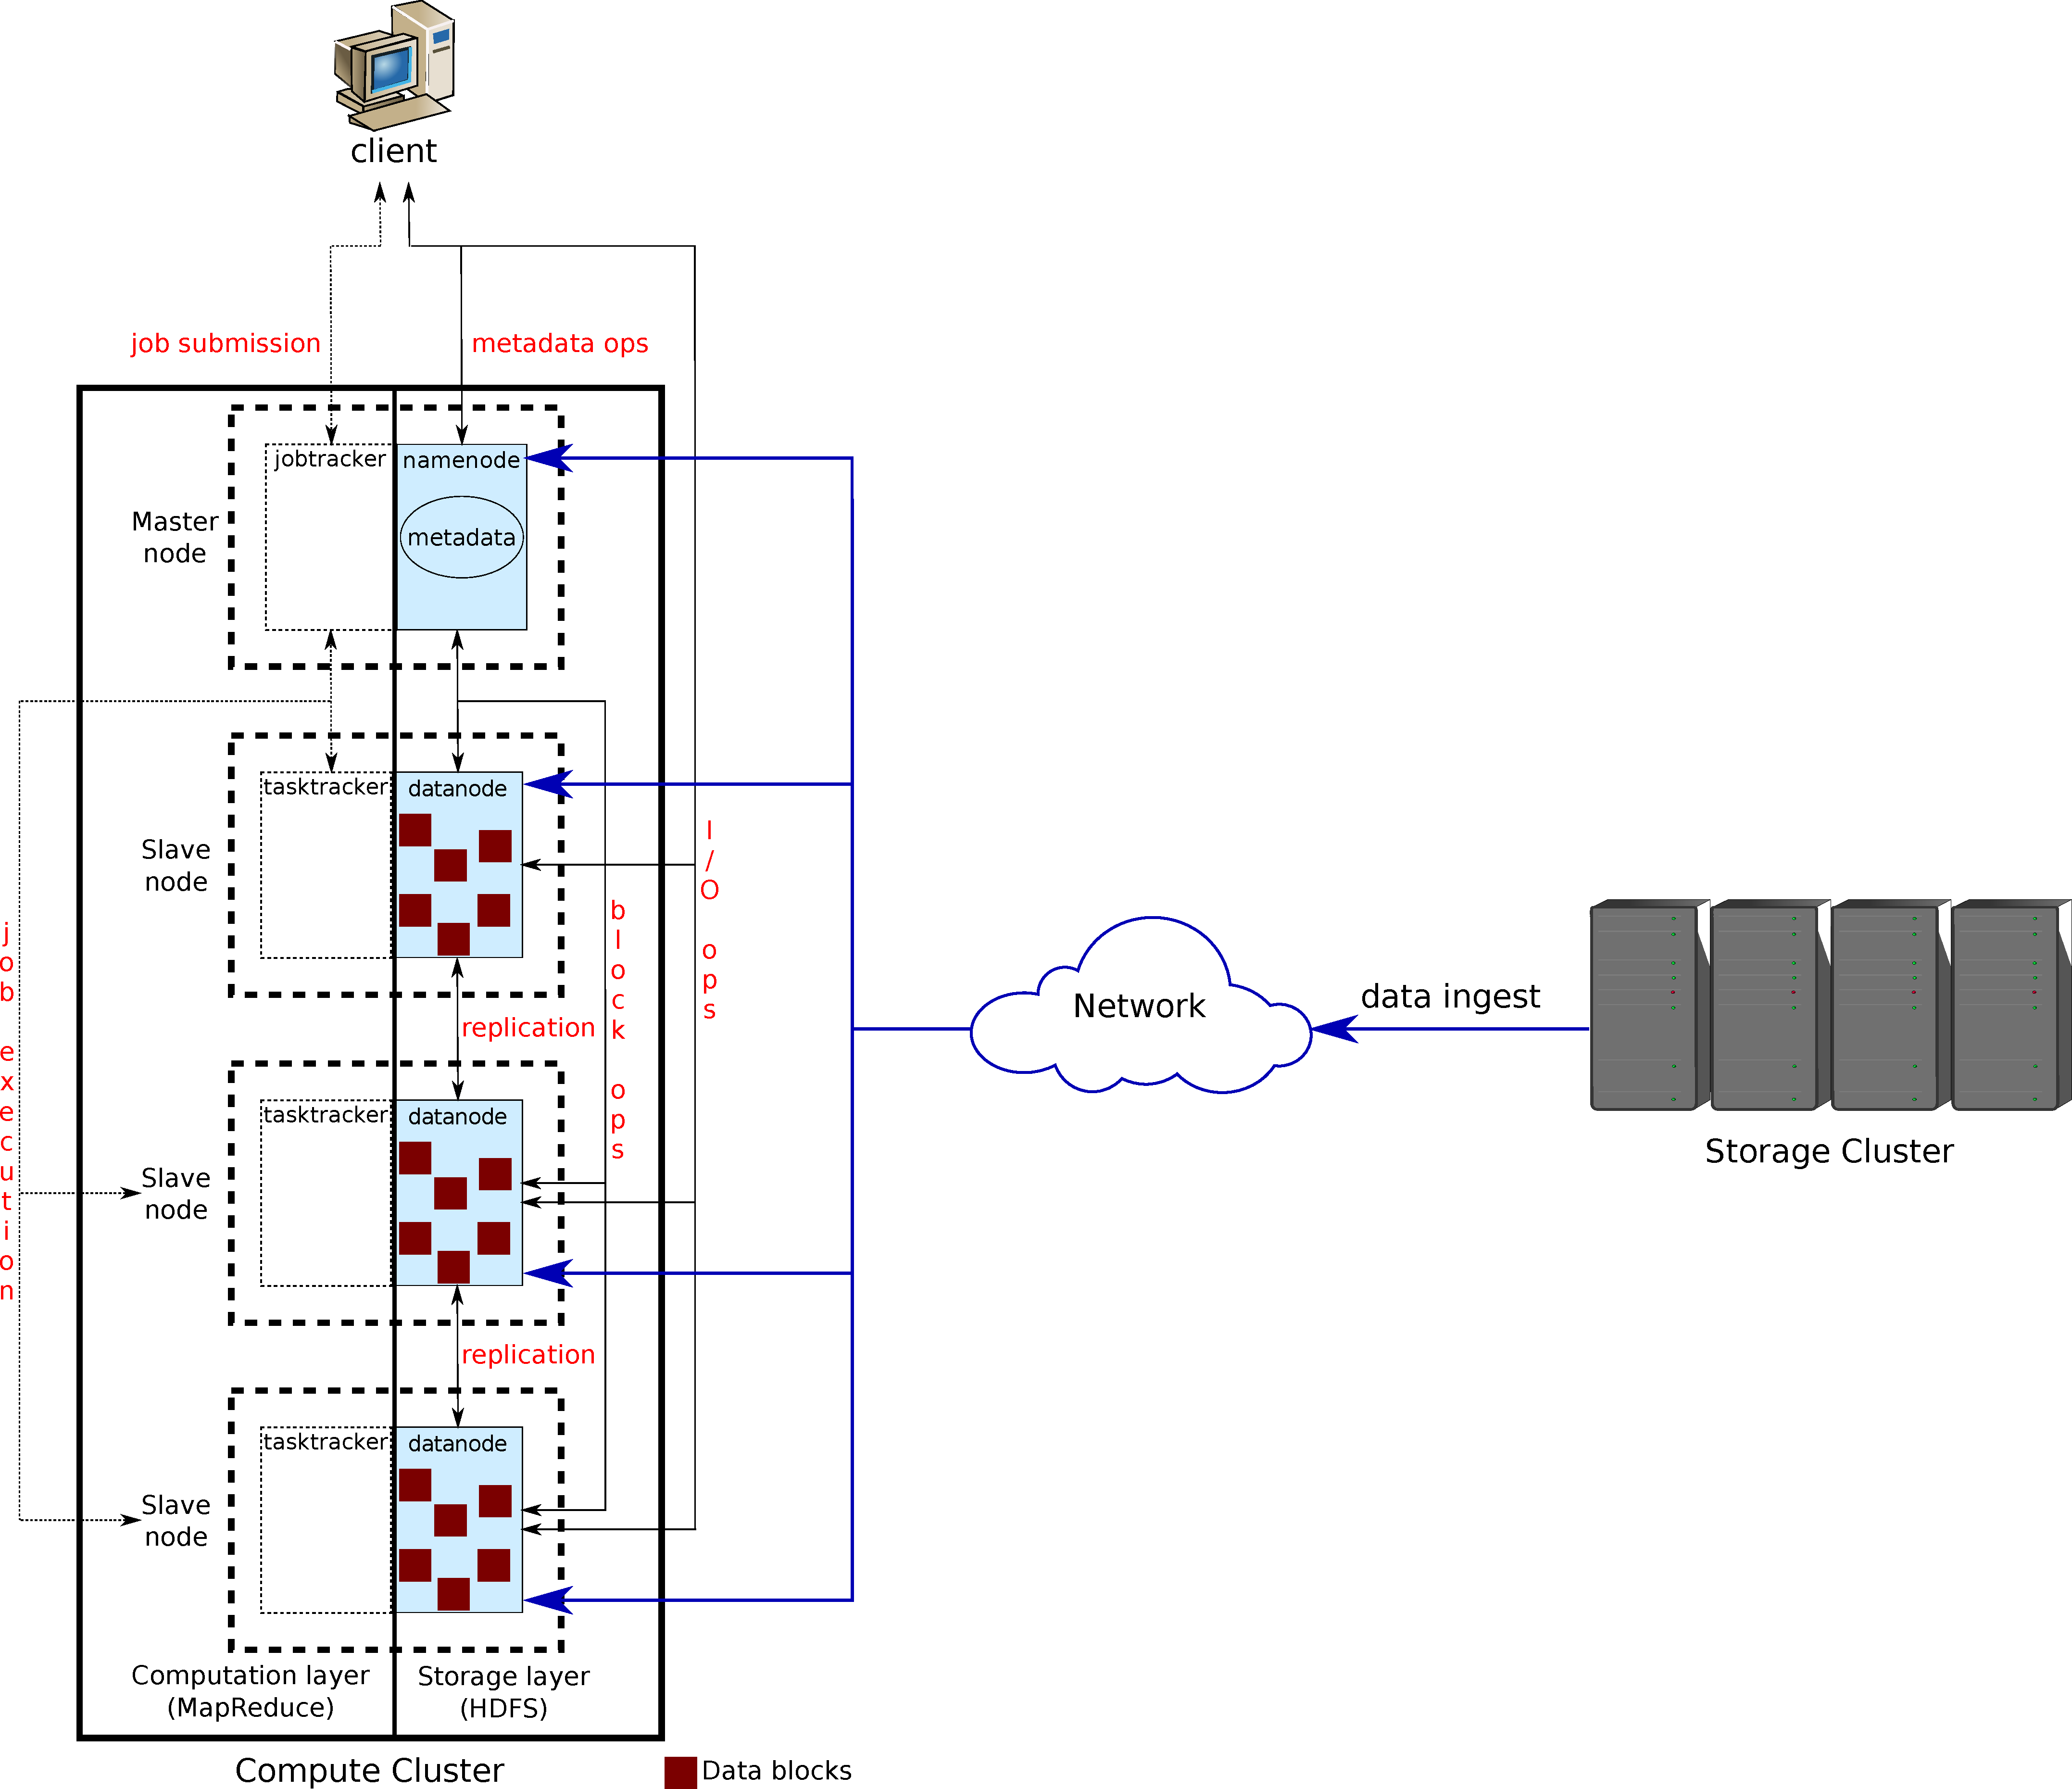
\includegraphics[width=\columnwidth, keepaspectratio]{hadoop_architecture.pdf}
\caption{Typical Hadoop Implementation Architecture}
\label{hadoop_arch}
\end{figure}

\subsection{Moving Hadoop Processes to Storage Cluster}
The biggest disadvantage of the typical approach presented in Figure~\ref{hadoop_arch}
is the need to transfer data between the storage and compute clusters before and
after a MapReduce application. Considering the size of data being moved, the network
interconnect can be easily maxed-out and the total energy consumption would increase
as system resources are utilized for data transfer.

The proposed approach implements Hadoop on the compute cluster. By doing so, the network
interconnect between separate clusters is completely eliminated and the compute cluster is
actually a storage cluster at the same time. Ceph stores object data and it is tied to
the datanode processes in Hadoop. This new architecture is shown in Figure~\ref{new_arch}.


\begin{figure}[!htbp]
\centering
\makebox[\textwidth]{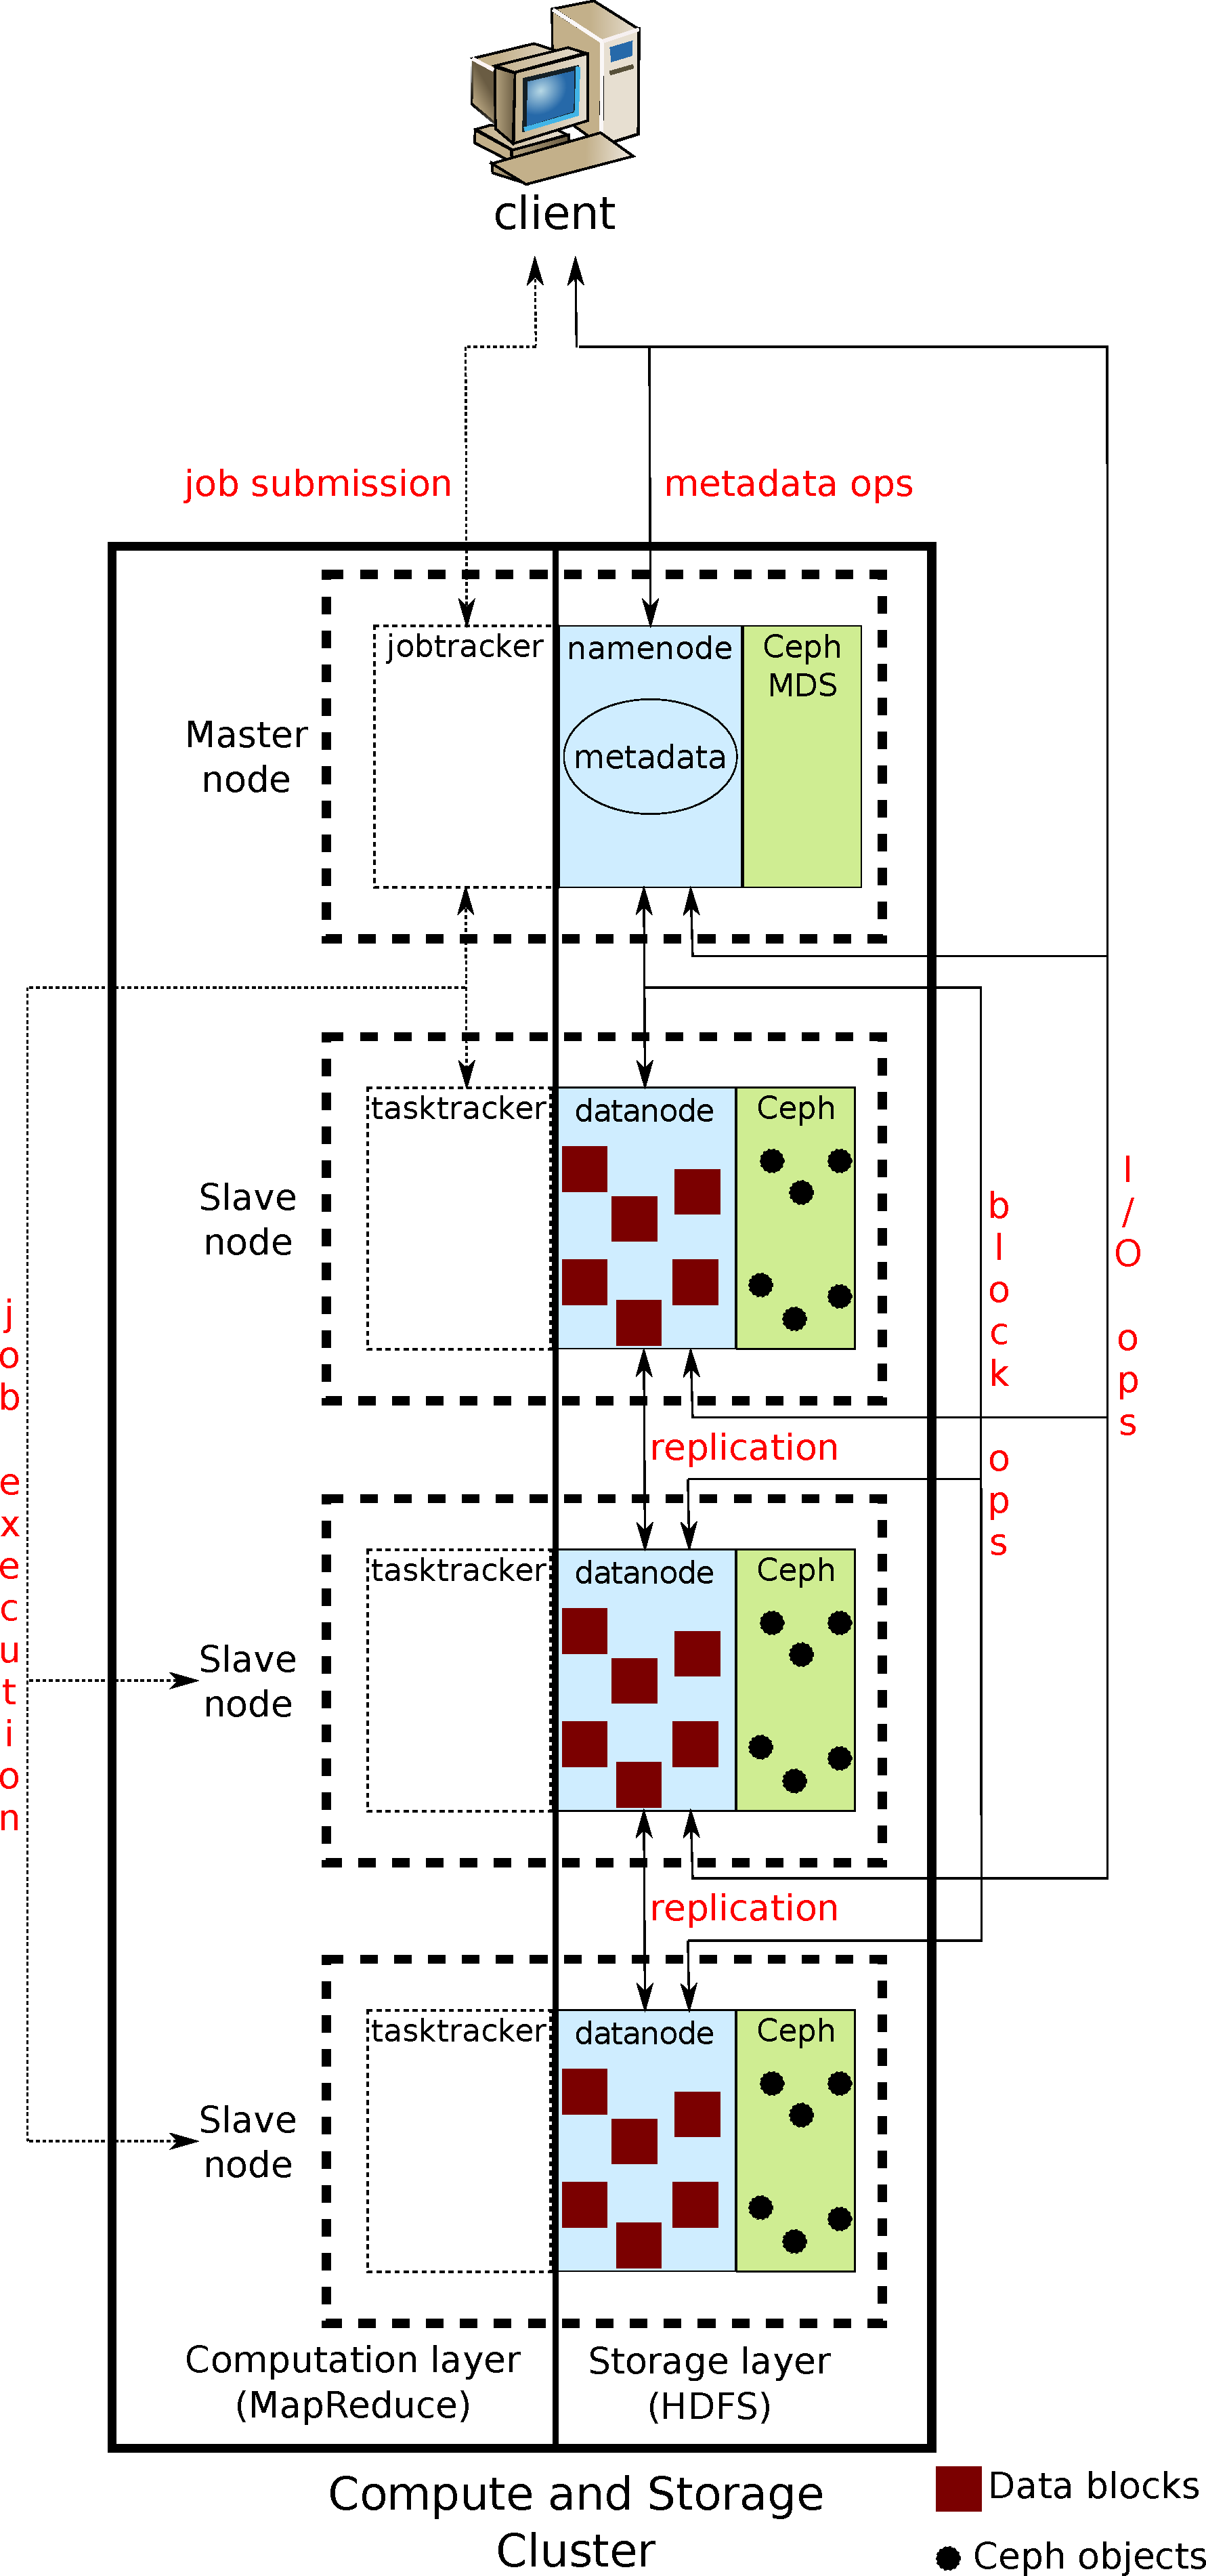
\includegraphics[scale=0.25, keepaspectratio]{hadoop_new.pdf}}
\caption{Proposed Hadoop Architecture}
\label{new_arch}
\end{figure}

\subsection{Initial Object Store Scan}
\label{initial_data_scan}
As shown in Figure~\ref{new_arch}, Ceph object store and Hadoop datanode processes are
tied together and there can be multiple methods to integrate Hadoop with the underlying Ceph storage system.
The most straight-forward approach would be to transfer object data directly from Ceph to HDFS.
Another approach can be using Ceph as the back-end storage of Hadoop and implementing
Hadoop data management policies there. Instead of these methods, this paper suggests
an alternative approach,~\textit{co-locating Ceph object store with Hadoop processes
on the same physical node and creating symbolic links in HDFS for data that already exists in
Ceph}. Creating symbolic links is a fairly fast operation, eliminates the need to transfer
data to HDFS and it will be discussed in Section~\ref{symlinks}. In order to create symbolic
links for the existing data in Ceph, certain properties of Ceph objects must be known. The
proposed approach makes these properties visible to HDFS, therefore makes Hadoop aware of
existing Ceph data, through~\textit{Global Information File}, which is created during the initial object store scan.

\begin{figure}[!htbp]
\centering
\makebox[\textwidth]{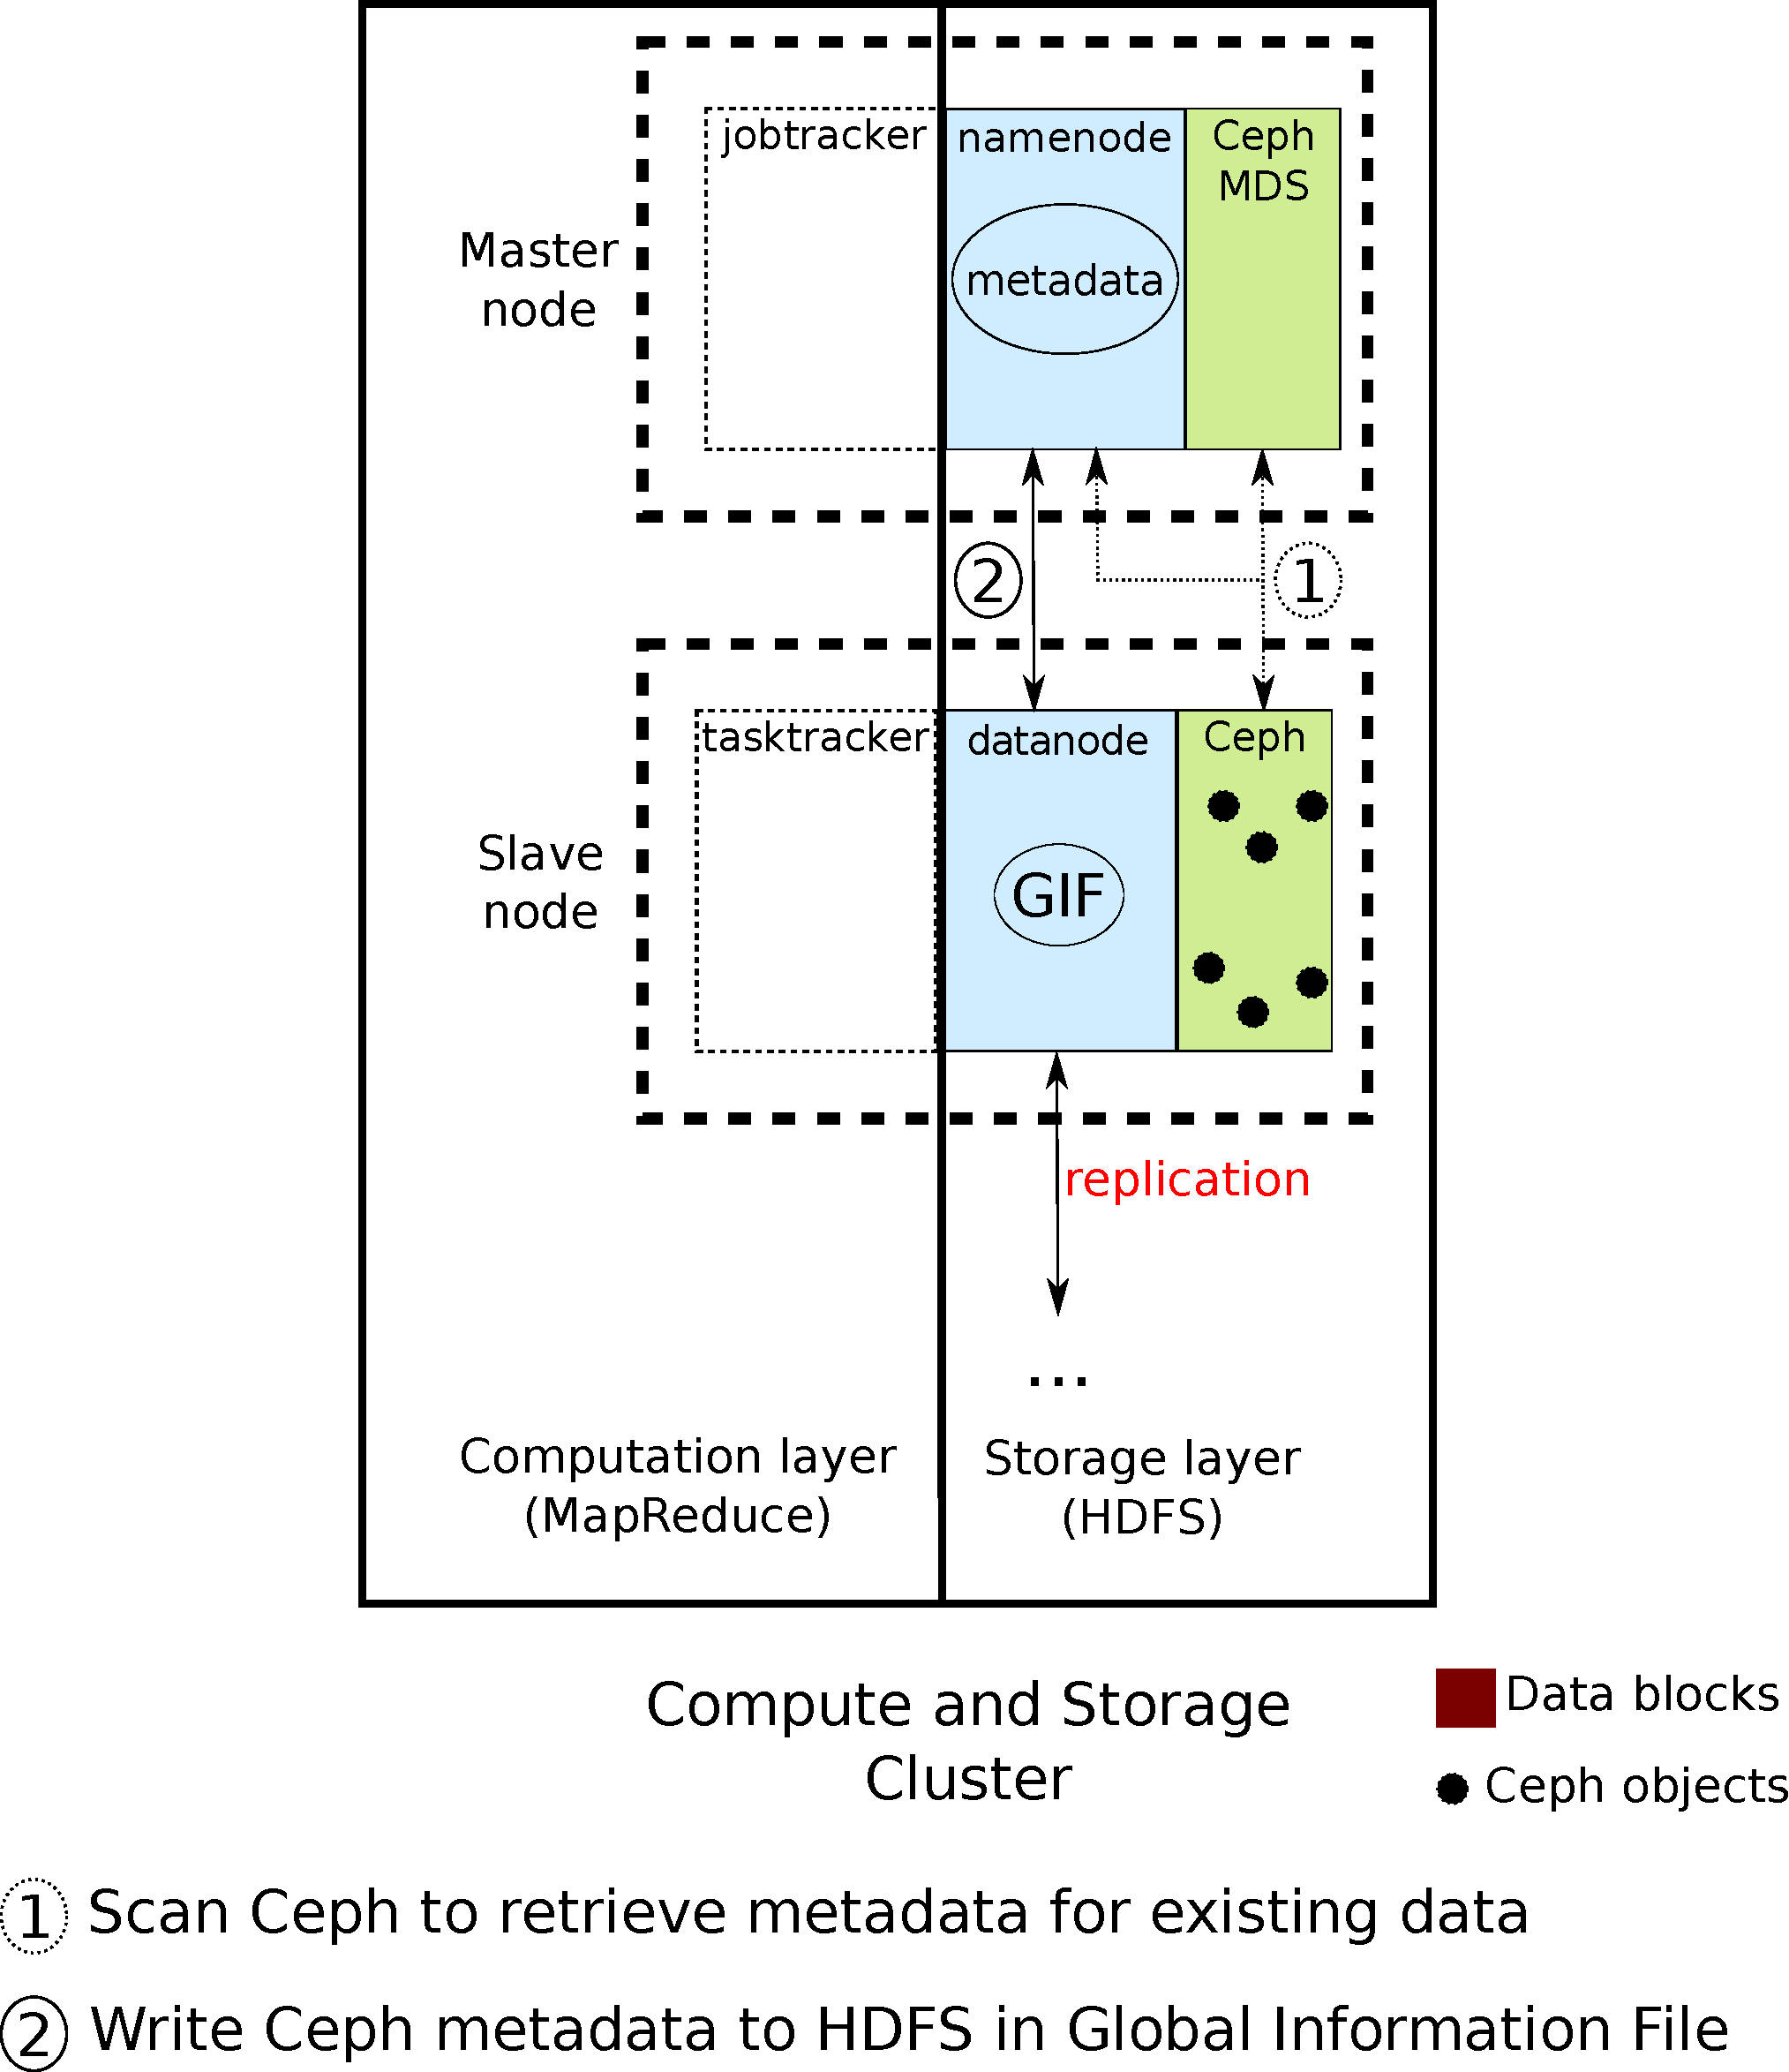
\includegraphics[scale=0.3, keepaspectratio]{initial_scan.pdf}}
\caption{Initial Integration of Ceph Object Store with Hadoop Datanodes}
\label{initial_scan}
\end{figure}

Figure~\ref{initial_scan} shows the process of initial object store scan. As a first step,
Hadoop namenode process communicates with Ceph Metadata Server (MDS) and it asks for the metadata
information of all the existing objects in Ceph. Metadata information provided by Ceph
to Hadoop is discussed in Section~\ref{global_file_contents}. After receiving the metadata from Ceph, Hadoop
namenode saves this information in the~\textit{Global Information File} and writes it
to HDFS (as if it is a regular file in HDFS), as shown in the second step in Figure~\ref{initial_scan}.
As mentioned earlier, Hadoop and Ceph preserve their stand-alone functionality in this
approach and that makes it possible to copy~\textit{Global Information File} to HDFS.

The procedure to create and distribute the~\textit{Global Information File} is less than ten seconds
for even 150 GB of data in Ceph and this is a one-time operation that is performed when Hadoop is initialized.
Hadoop trusts the information in the~\textit{Global Information File} and once Hadoop daemons are successfully
started, Ceph daemons do not even have to run anymore. If new data is available in Ceph, Ceph can be scanned
again to regenerate the~\textit{Global Information File}. Hadoop daemons will pick up the updated
information after a restart. It is important to note that incrementally updating the~\textit{Global Information File}
with each write operation in a write-heavy workload will be expensive as the existing data blocks will be scanned over and over
again. This work is geared towards updating the~\textit{Global Information File} asynchronously on already existing
data in a write-once-read-many workload, which is the optimal use case for MapReduce applications.

\subsection{Contents of the Global Information File}
\label{global_file_contents}
The~\textit{Global Information File} is created during the initial data scan, as discussed in Section~\ref{initial_data_scan},
and it is crucial for the integration of Hadoop and Ceph object store. Following is the summary of information
stored in the~\textit{Global Information File}.
\begin{itemize}
\item~\textit{File names} and~\textit{pre-calculated block names} are used by Hadoop to identify
objects that already exist in Ceph. Pre-calculated block names are formed by hashing object name, object
location and replication level provided by Ceph. If a block does not follow this naming convention,
Hadoop will treat that block as a regular HDFS block and this will make it possible for Hadoop to
preserve its normal functionality. Meanwhile, not all Ceph objects have to be visible to Hadoop.
Any object that is not scanned will not be in the~\textit{Global Information File} and therefore,
will not be visible to Hadoop applications. Any application or user can read the~\textit{Global
Information File} and find the~\textit{pre-calculated block name} using a~\textit{file name}.
\item~\textit{Replica locations} are of critical importance. As it is the case with any other storage
system, Ceph has its own replica placement policy and it is preserved in the proposed approach,
as the ultimate goal is to perform in-place computation on existing data without moving it anywhere
else.
\item~\textit{Absolute paths} are necessary while creating symbolic links to already existing Ceph data from
Hadoop.
\item As this work does not ingest any data into HDFS, Hadoop does not know about the sizes of
existing Ceph objects. The~\textit{file sizes} are fed from the~\textit{Global Information File} to
Hadoop for MapReduce operations to work properly.
\end{itemize}

Table~\ref{gif_example} shows an example of two rows from the~\textit{Global Information File}.

\begin{table}[!htbp]
 \begin{center}
 \resizebox{\columnwidth}{!}{%
  \begin{tabular}{|l|l|l|l|l|} \hline
\textbf{File Name} & \textbf{Pre-calculated Block Name} & \textbf{Replica Location}  & \textbf{Absolute Path}  & \textbf{File Size}\\ \hline
testfile1 & blk\_582040001401 & node1 & /mnt/ceph/dir1/obj1 & 65536\\ \hline
testfile2 & blk\_381980001533 & node4 & /mnt/ceph/dir1/obj2 & 65536\\ \hline
  \end{tabular}%
 }
 \end{center}
 \caption{Example Rows from the~\textit{Global Information File}}
 \label{gif_example}
\end{table}

\subsection{Creating Symbolic Links}
\label{symlinks}
Once the~\textit{Global Information File} is written to HDFS and distributed to each datanode,
datanodes can read metadata from the~\textit{Global Information File} and create symbolic
links for the existing Ceph data accordingly. This procedure is illustrated in Figure~\ref{symbolic_lins}.

\begin{figure}[!htbp]
\centering
\makebox[\textwidth]{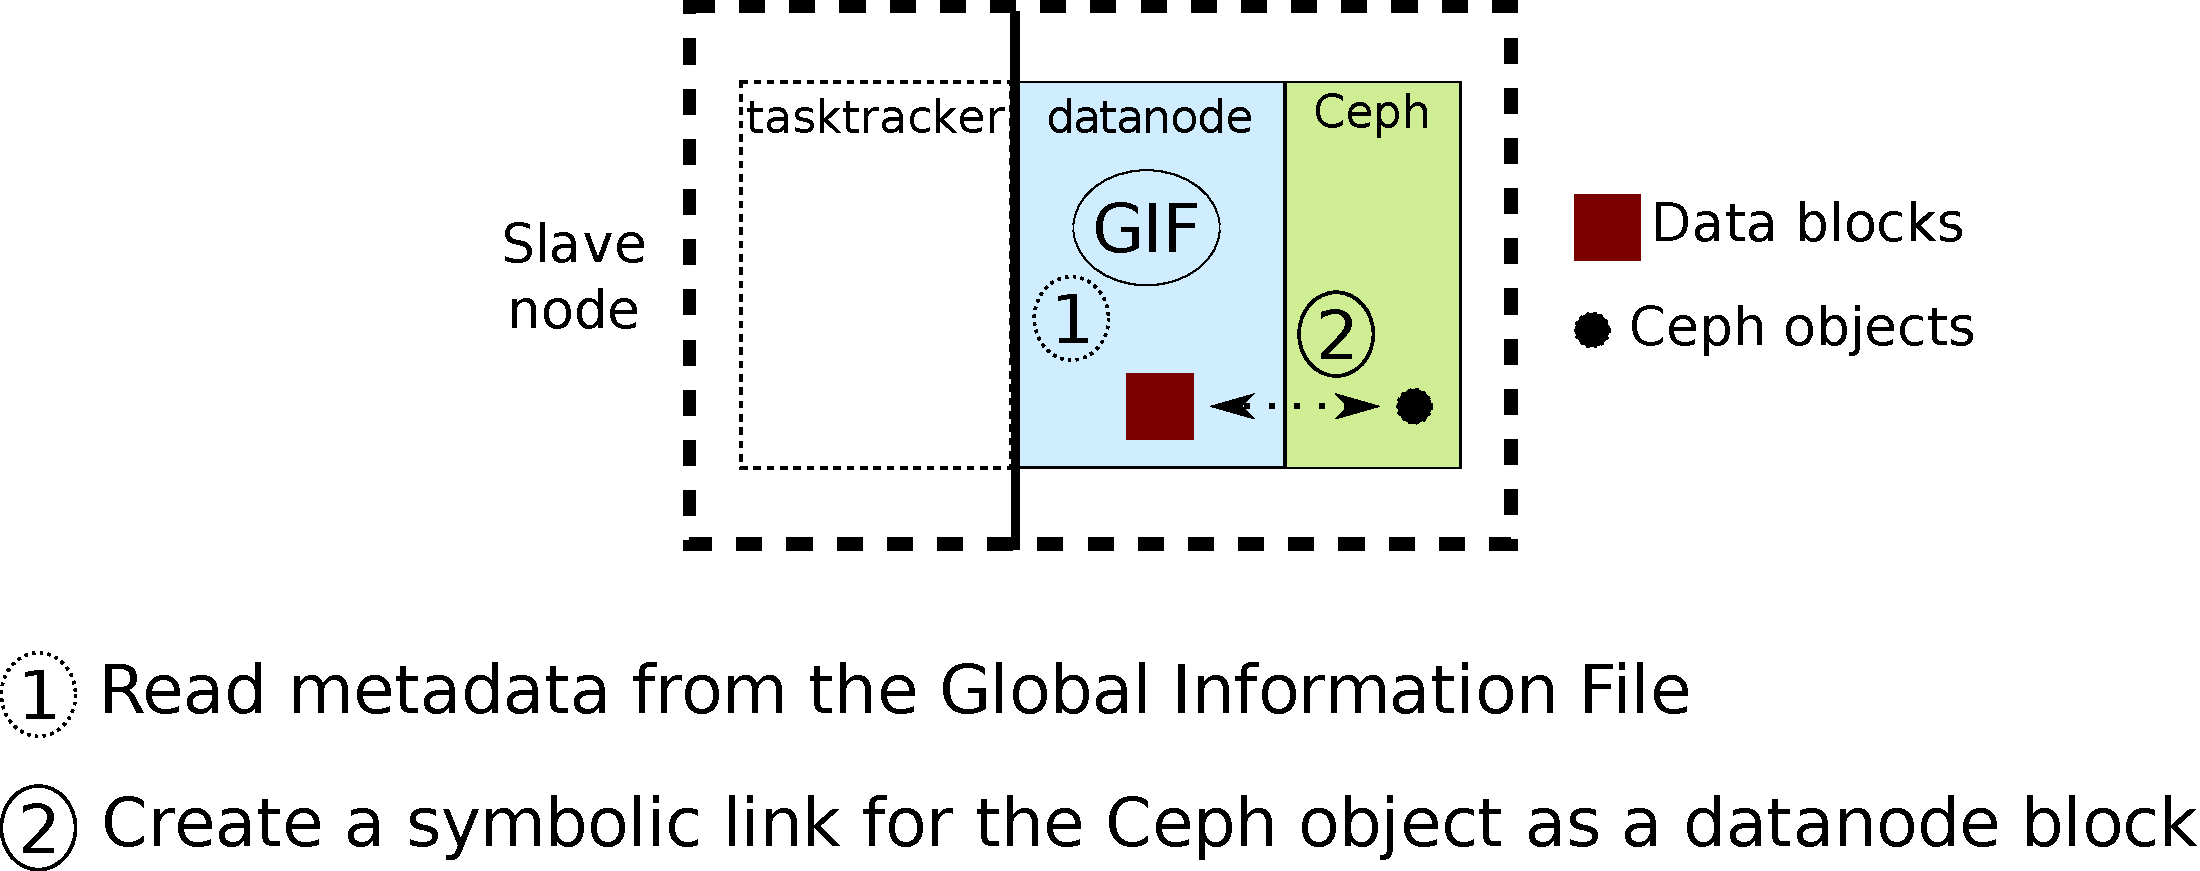
\includegraphics[scale=0.3, keepaspectratio]{symbolic_lins.pdf}}
\caption{Creating Symbolic Links for Existing Ceph Data}
\label{symbolic_lins}
\end{figure}

As part of this work, symbolic link creation function in Hadoop is modified to accept two arguments;~\textit{file name}
and~\textit{replica location}. At first, datanode reads a row from the~\textit{Global Information File}. In order to create a
symbolic link, the datanode needs to know the~\textit{absolute path} of the Ceph object on that node (i.e. /mnt/ceph/dir1/obj1)
and the~\textit{pre-calculated block name} (i.e. blk\_381980001533) that will be assigned to the newly created symbolic link.
Both of these parameters can be found from the~\textit{Global Information File} by finding the row that
matches with the given~\textit{file name} (i.e. testfile1) and~\textit{replica location} (i.e. node1). After retrieving this information,
the datanode creates the symbolic links and changes its metadata; such that the size of the symbolic link
is equal to the actual size of the object. This is accomplished by using the~\textit{file size} (i.e. 65536) information
from the~\textit{Global Information File}. Setting the correct~\textit{file size} is important as MapReduce
operations reading data through these symbolic links need to know the exact size of the data for the correctness
of I/O operations.

It is important to note that symbolic links are created for data blocks only. Since data is not ingested
into HDFS in the proposed approach, Hadoop creates a metadata block of negligible size for a Ceph object.
Metadata creation is dominated by checksum calculation and reading no data from Ceph means having an empty
checksum. Additionally, the~\textit{Global Information File} has most of the metadata needed for symbolic link
creation. As a result, Hadoop metadata block creation overhead is negligible. Checksum implementation is left
as a future work item as discussed in Section~\ref{conclusions}.

Another important design decision is to disable datanode
block scans. Hadoop datanodes are responsible for scanning data blocks they own and they report bad
blocks to the namenode. Symbolic links created for existing Ceph data are detected and invalidated during block scans
and to prevent this from happening, datanode block scans have to be disabled. Configuration changes for
datanode block scans are described in Section~\ref{hadoopconfs}. Modifying the datanode block scan in order to
prevent it catching symbolic links while resuming its normal functionality is also left as a future work item,
as discussed in Section~\ref{conclusions}.

\subsection{Performing a MapReduce Application}
At this point, initial data scans and symbolic links creations are done and any MapReduce application can be executed
on Ceph objects as if they are located in HDFS. Since the proposed approach ingests no data to HDFS and creates
symbolic links only for the Ceph objects located in the same physical node, that means mappers have to work local
data. Therefore, the scheduling policy of mappers has to be modified. This is accomplished by changing
MapReduce task scheduler code; such that, it assigns local map tasks if a MapReduce operation is executed on
symbolic links (existing Ceph data). This also requires MapReduce split size to be exactly the same with the split
size of the underlying storage systems. Configuration changes for the MapReduce split size are also described in
Section~\ref{hadoopconfs}.

\section{Performance Evaluation}
\label{sec-performance}
\label{results}
This section describes the experimental setup first followed by explanation of the
performance evaluation tests and the discussion of the test results.

\subsection{Experimental Setup}
Experimental evaluations are conducted using five Google Compute Engine~\cite{gce}
instances. Each instance has two Intel Sandy Bridge vCPUs, 7.5 GB of memory and 250 GB
of storage. The instance are grouped in an instance group in~\textit{us-central1-a} zone
to simulate a cluster consisting of five nodes. Each instance has internal and external
network access configured and passwordless SSH connection enabled to other instances.

\subsection{Hadoop Configuration Parameters}
\label{hadoopconfs}
In order to have a fair comparison against stock Hadoop implementation, the configuration
parameters (dfs and mapreduce) are preserved during all performance evaluation tests.
Table~\ref{hadoopparams} shows the configuration parameters used for the experimental evaluations.

\begin{table}[!htbp]
 \begin{center}
  \resizebox{\columnwidth}{!}{%
  \begin{tabular}{|l|l|} \hline
\textbf{Hadoop Configuration Parameter} & \textbf{Values} \\ \hline
dfs.replication                     & 2 or 3 \\ \hline
dfs.datanode.max.receivers          & 81920000 \\ \hline
dfs.datanode.socket.write.timeout   & 0 \\ \hline
dfs.datanode.scan.period.hours      & -1 \\ \hline
mapred.child.java.opts              & -Xmx6144m \\ \hline
mapred.task.timeout                 & 0 \\ \hline
mapreduce.map.output.compress       & true \\ \hline
mapreduce.map.output.compress.codec & org.apache.hadoop.io.compress.GzipCodec \\ \hline
mapred.child.ulimit                 & unlimited \\ \hline
mapred.min.split.size               & matches underlying storage \\
                                    & (see below for explanation) \\ \hline
  \end{tabular}%
 }
 \end{center}
 \caption{Hadoop Configuration Parameters}
 \label{hadoopparams}
\end{table}

Details on these configurations are available in the Hadoop documentation~\cite{hadoopconf}.
There are two important configuration parameters that should be further explained here -
~\textit{dfs.datanode.scan.period.hours} and~\textit{mapred.min.split.size}. Since the
proposed method in this work does not really write any data to HDFS; but, rather creates
symbolic links to existing data, datanode scans catch these links. In order to make Hadoop
work properly with symbolic links, datanode scans are disabled. Additionally, the minimum
split size of MapReduce,~\textit{mapred.min.split.size}, matches that of the underlying
storage system, so that they work on the same number of splits for a fair comparison.

\subsection{Performance Tests}
Experimental evaluations are conducted using Hadoop 1.1.2 stable version and
Ceph 0.94(Hammer) release. The benchmarks used are~\textit{Grep}~\cite{hadoopgrep},
~\textit{Wordcount}~\cite{hadoopwordcount},~\textit{TestDFSIO}~\cite{hadooptestdfsio}
and~\textit{TeraSort}~\cite{hadoopterasort}. These benchmarks are commonly used to evaluate
Hadoop applications (i.e. Tantisiriroj et al.~\cite{Tantisiriroj:2011:DDF:2063384.2063474}
uses~\textit{Grep}, Maestro~\cite{6217451} uses~\textit{Wordcount}, Kulkarni et
al.~\cite{hadoopyarnprogress} uses~\textit{TestDFSIO} and Ananthanarayanan et
al.~\cite{Ananthanarayanan:2009:CAW:1855533.1855548} uses~\textit{TeraSort})
and they have different characteristics in terms of the size of data
they use or generate.~\textit{Grep} searches for a pattern in a potentially large file
and generates a small set of output containing matches.~\textit{Wordcount} is similar,
but it generates much larger output.~\textit{TestDFSIO} and~\textit{TeraSort} generate
their own input data and perform their tests on the generated data.~\textit{TestDFSIO}
performs basic I/O operations (read and write in this work) on the generated data. Number of
files to perform I/O and size of the I/O operation are configurable parameters of~\textit{TestDFSIO}.
~\textit{TeraSort} sorts data generated by the~\textit{TeraGen} benchmark and optionally, sorted
data can be verified with~\textit{TeraValidate} benchmark. The size of data produced by~\textit{TeraGen}
is also a configurable parameter.

\subsection{Test Results}
Table~\ref{testparams} shows the parameters used during the evaluations.

\begin{table}[!htbp]
 \begin{center}
  \resizebox{\columnwidth}{!}{%
  \begin{tabular}{|l|l|} \hline
\textbf{Test Parameter} & \textbf{Values} \\ \hline
Total number of nodes    & 3, 5 \\ \hline
Replication levels       & 2 replicas, 3 replicas \\ \hline
Benchmarks               & Grep, Wordcount, TestDFSIO, TeraSort \\ \hline
Input size per file      & Grep (25 MB, 242 MB, 2.4 GB) \\
                         & Wordcount (29 MB, 286 MB, 2.8 GB) \\
                         & TestDFSIO (500 MB, 5000 MB, 15000 MB, 25000 MB, 50000 MB) \\
                         & TeraSort (1 GB, 10 GB, 50 GB) \\ \hline
  \end{tabular}%
 }
 \end{center}
 \caption{Test Parameters}
 \label{testparams}
\end{table}

\subsubsection{Grep}
\label{greptest}
The results of the experimental evaluations for the~\textit{Grep} benchmarks are discussed first.
This benchmark searches for a pattern in a given file and extracts the occurrences
of the given phrase to the resulting output file - so, it generates output much smaller
in size compared to its input.

In this test case, 100 files that are equal to each other in size (25 MB, 242 MB or 2.4 GB)
are generated first. Stock Hadoop creates these files in HDFS and writes data to each.
In the proposed implementation, these files already exist in Ceph and the only requirement
is to make Hadoop aware of these existing files through symbolic links during its initialization. 
Following the data creation,~\textit{Grep} benchmark is executed on the newly created data.
The test steps outlined above are performed for both 3 nodes with 2 replicas and 5 nodes with
3 replicas.

\begin{figure}[!htbp]
\centering
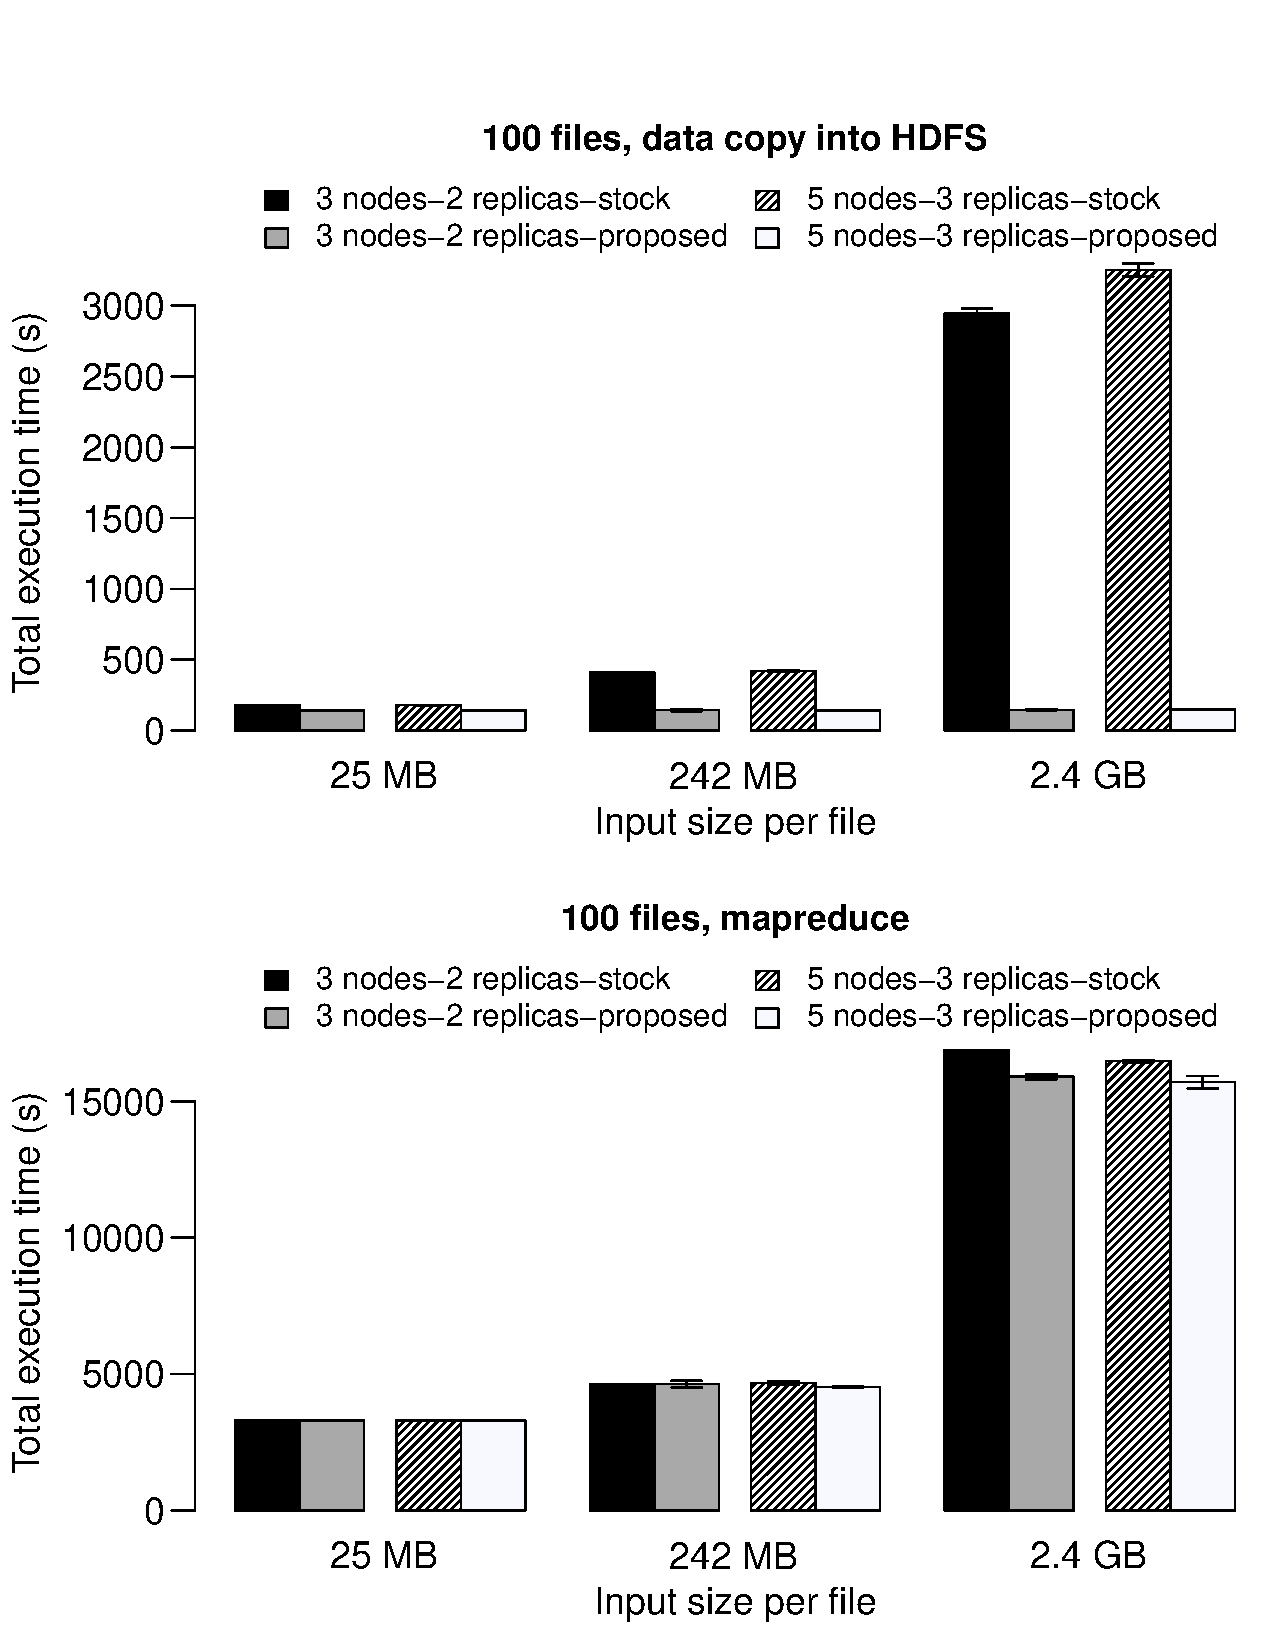
\includegraphics[width=\columnwidth, keepaspectratio]{result1.pdf}
\caption{Evaluation results for~\textit{Grep}}
\label{grepres}
\end{figure}

The upper sub-plot of Figure~\ref{grepres} shows the measurements of the total time it
takes to copy data into HDFS. As can be inferred, the proposed Hadoop implementation
takes significantly less time than stock Hadoop to copy data into HDFS; because, no
data is actually ingested into HDFS. As the input size per file is
increased from 25 MB to 2.4 GB, the time it takes to copy data into HDFS increases
for stock Hadoop. As no data is written to HDFS, that time stays constant
for the proposed implementation. An improvement of 95\% in terms of 
initial data copy performance is achieved and as the input size becomes larger, this improvement
will become even higher. Another conclusion from Figure~\ref{grepres} is that the
number of replicas or total storage nodes in the system does not have a significant
effect on the performance of the data copy phase.

Improving the performance of the MapReduce phase is not a primary goal of this work, as the
optimizations are targeted for the initial data copy phase; but, as the input size per file
becomes larger (i.e. 2.4 GB), nearly 5\% of improvement in MapReduce performance is observed
due to data-compute locality. This is achieved by using the object storage system to identify
replicas and force Hadoop to co-locate compute threads with the appropriate replica. Note that,
there are a variety of existing techniques to co-locate data and compute in Hadoop; but, they
do not help improving the performance of data copy phase, which is the primary goal of this work.
Similar to the data copy phase, the number of replicas or total storage nodes does not have a
significant effect on the performance of the MapReduce phase.

\subsubsection{Wordcount}
This section gives the evaluation results for the~\textit{Wordcount} benchmark.
~\textit{Wordcount} counts the number of occurrences of each word in a given file and
saves these numbers in an output file that is of similar size as the input.

Test parameters of the~\textit{Wordcount} benchmark are exactly the same
with those used for the~\textit{Grep} benchmark in Section~\ref{greptest};
except for the file sizes (29 MB, 286 MB or 2.8 GB per file).

\begin{figure}[!htbp]
\centering
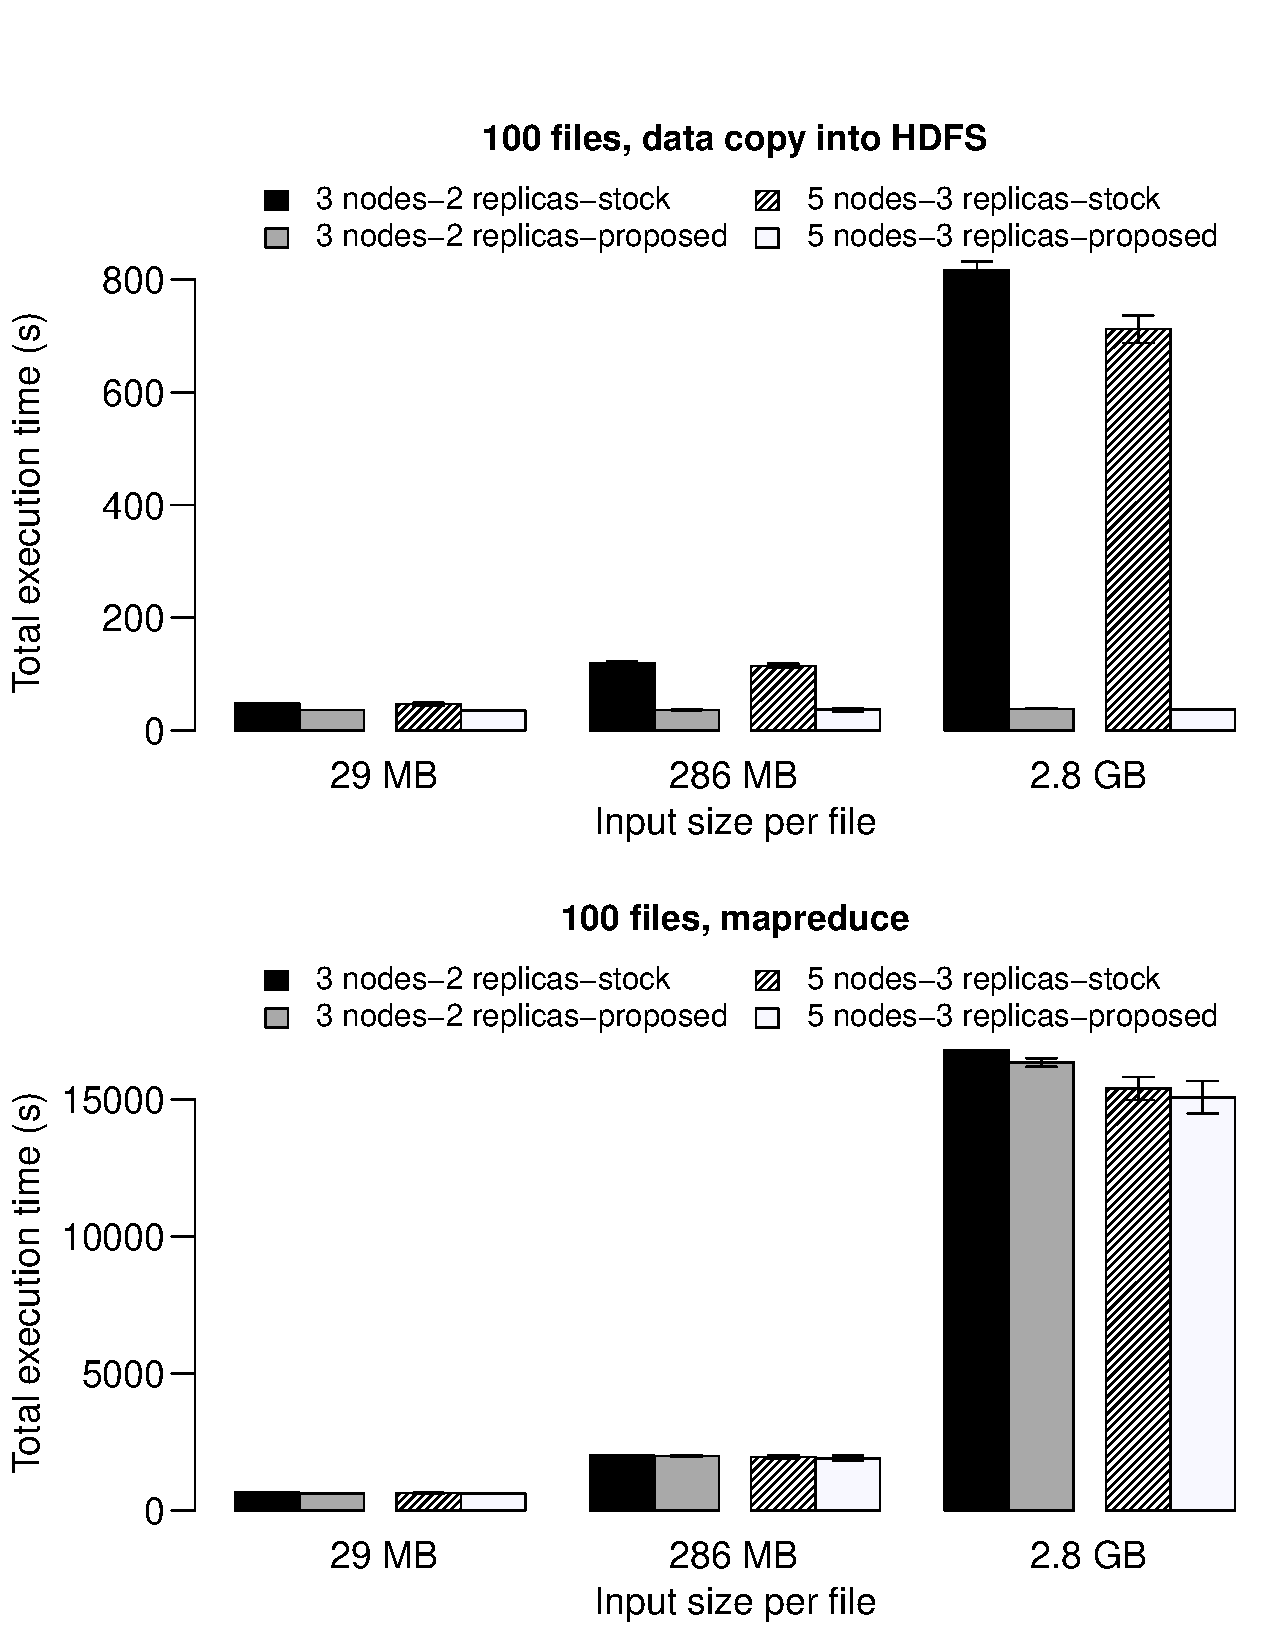
\includegraphics[width=\columnwidth, keepaspectratio]{result2.pdf}
\caption{Evaluation results for~\textit{Wordcount}}
\label{wordcountres}
\end{figure}


The upper sub-plot of Figure~\ref{wordcountres} shows the total time to copy data into HDFS.
The performance improvement is nearly 95\%, similar to the improvement observed for
the~\textit{Grep} benchmark in Section~\ref{greptest}. Additionally, increasing the
input size per file, the number of replicas or total storage nodes has similar impacts
and MapReduce performance is improved by nearly 5\% as data and computation are co-located,
with the number of replicas or storage nodes having no significant effect.

\subsubsection{TestDFSIO}
This section presents the experimental evaluation results for the~\textit{TestDFSIO}
benchmark. This benchmark generates its own input with its~\textit{write} option using
MapReduce, rather than the traditional data ingest method. It is possible to specify
the number and size of files to generate with~\textit{TestDFSIO} benchmark. In this test
case,~\textit{TestDFSIO} does not generate any input data, because its input already exists
in the system. When a~\textit{TestDFSIO} run is completed, it dumps statistics about the
benchmark performance (throughput, execution time, io rate etc.).

For the sake of simplicity and as the number of input files will not have a significant effect
on the outcome of~\textit{TestDFSIO} tests,~\textit{TestDFSIO} benchmark is tested with a single
file and the file size is varied between 500 MB and 50000 MB. Stock Hadoop creates these files with
the~\textit{write} option of~\textit{TestDFSIO} and then performs a read operation on them. The
implementation presented in this work performs a zero-length write that sets up symbolic links to
already existing data, followed by a read operation. These test steps are performed for both
3 nodes with 2 replicas and 5 nodes with 3 replicas.

\begin{figure}[!htbp]
\centering
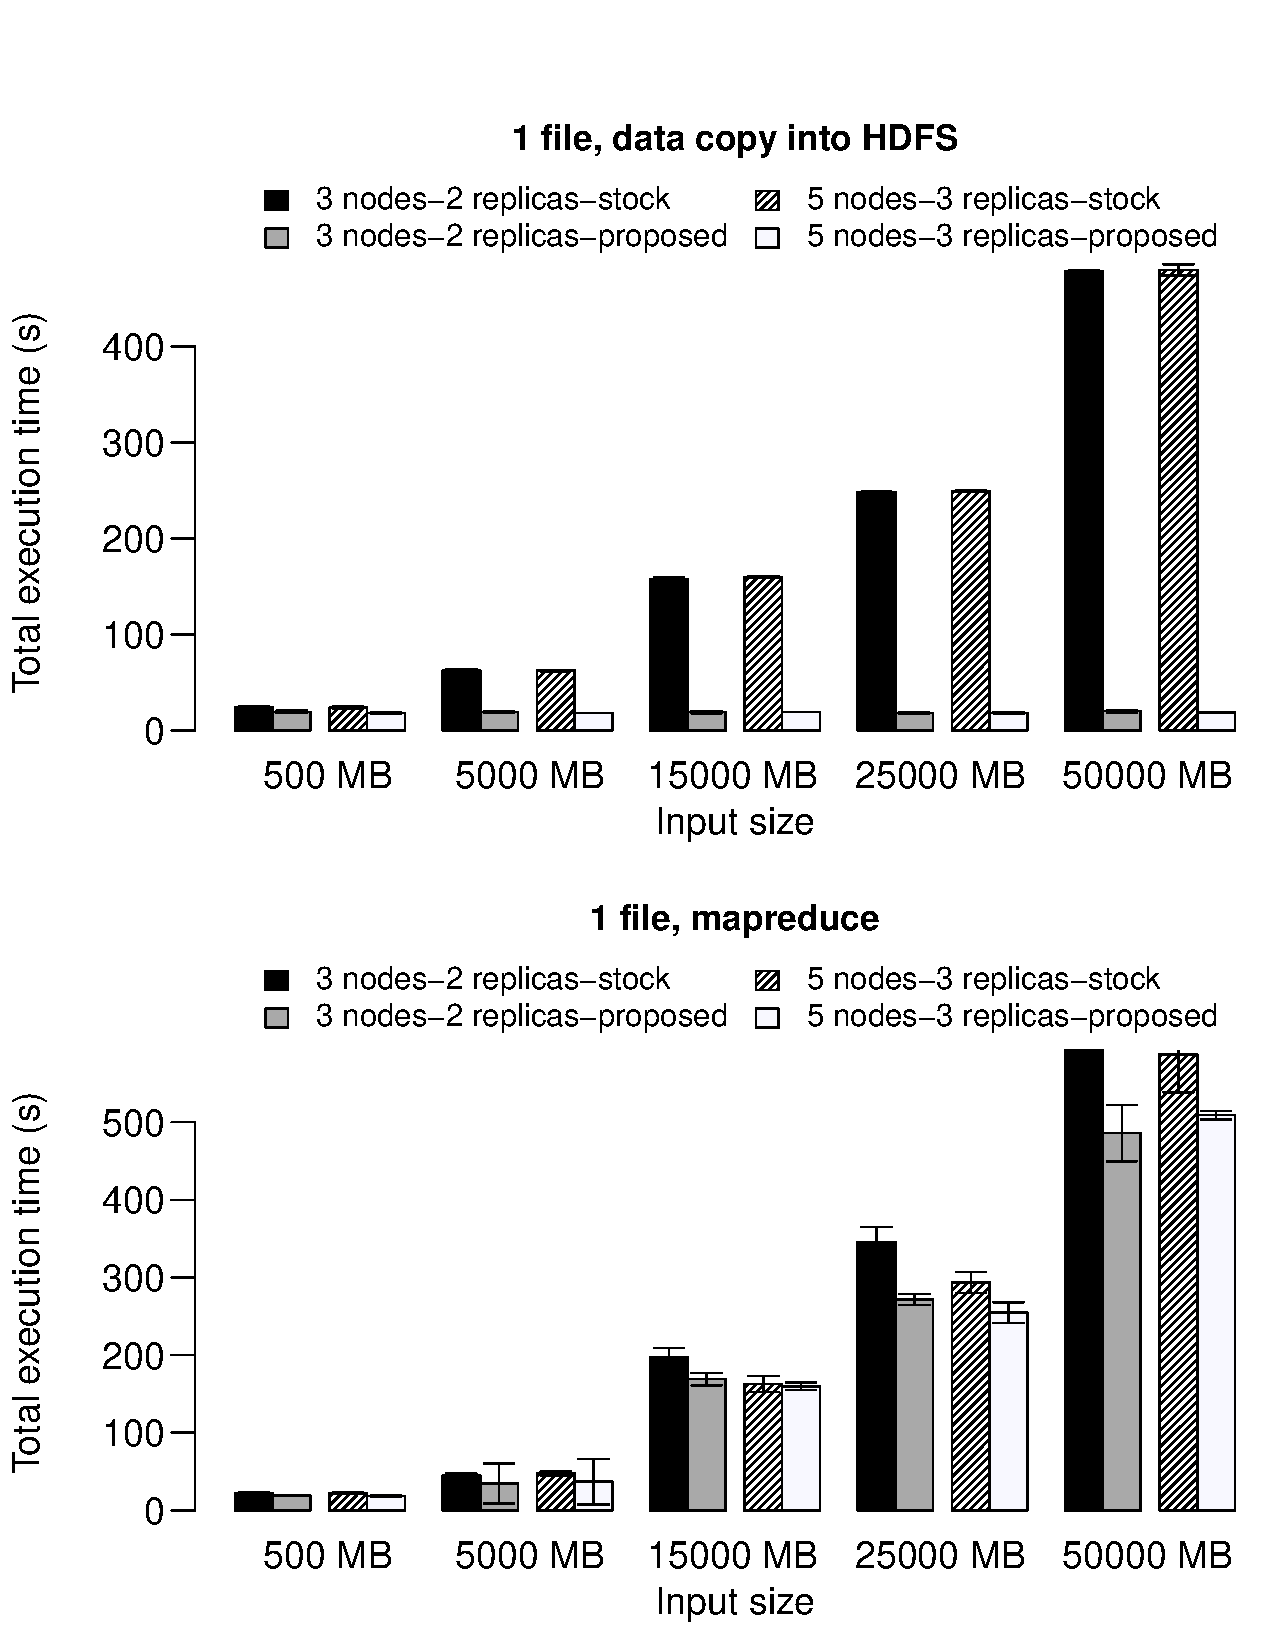
\includegraphics[width=\columnwidth, keepaspectratio]{result3.pdf}
\caption{Evaluation results for~\textit{TestDFSIO}}
\label{testdfsiores}
\end{figure}

Figure~\ref{testdfsiores} shows the data copy and MapReduce performance of the proposed implementation
compared with that of stock Hadoop. First conclusion to draw is that regardless of the input data size
and the number of replicas and storage nodes, our Hadoop implementation spends the same amount of time
for the initial ingestion of data. On the other hand, the time it takes for stock Hadoop to create the
data with the~\textit{write} option of~\textit{TestDFSIO} increases as the file size is increased
from 500 MB to 50000 MB. At 50000 MB, the proposed implementation achieves a 96\% improvement over the stock
Hadoop implementation in terms of data copy performance. For the MapReduce phase, as the file size
is increased, our Hadoop implementation performs better when compared to stock Hadoop.
Since local map tasks are used, which means data and computation are co-located, the time it takes
to shuffle mapper outputs to reducers is much smaller. Additionally,~\textit{TestDFSIO}
MapReduce phase is dominated by reading the generated data which happens totally local,
making the MapReduce improvement more apparent. As a result, MapReduce performance is improved
by nearly 20\% with the number of replicas or storage nodes having no significant effect.
~\textit{TestDFSIO} test results are highly variant and this is a known issue with
the~\textit{TestDFSIO} benchmark~\cite{hdfs941}.

\subsubsection{TeraSort}
Finally, this section presents the experimental evaluation results for the~\textit{TeraSort} benchmark.

Similar to the~\textit{TestDFSIO} benchmark,~\textit{TeraSort} generates its own input
with the~\textit{TeraGen} benchmark using MapReduce, rather than the traditional
data ingest method. The input data generated by~\textit{TeraSort} consists of 100-byte rows.
It is possible to specify the size of input data to be generated with~\textit{TeraGen}. While
evaluating the proposed changes,~\textit{TeraSort} does not generate any input data as its input
already exists.

The input size for~\textit{TeraSort} benchmark is varied between 5 GB, 10 GB and 50 GB during
the performance evaluations. Stock Hadoop implementation creates files of these sizes with the
~\textit{TeraGen} benchmark and then sorts them with~\textit{TeraSort}. Our Hadoop implementation performs
a zero-length write when~\textit{TeraGen} is executed and creates symbolic links to already existing data.
~\textit{TeraSort} sorts generated data and finally~\textit{TeraValidate} is executed to validate the
sorted data. This test case is performed for both 3 nodes with 2 replicas and 5 nodes with 3 replicas.

\begin{figure}[!htbp]
\centering
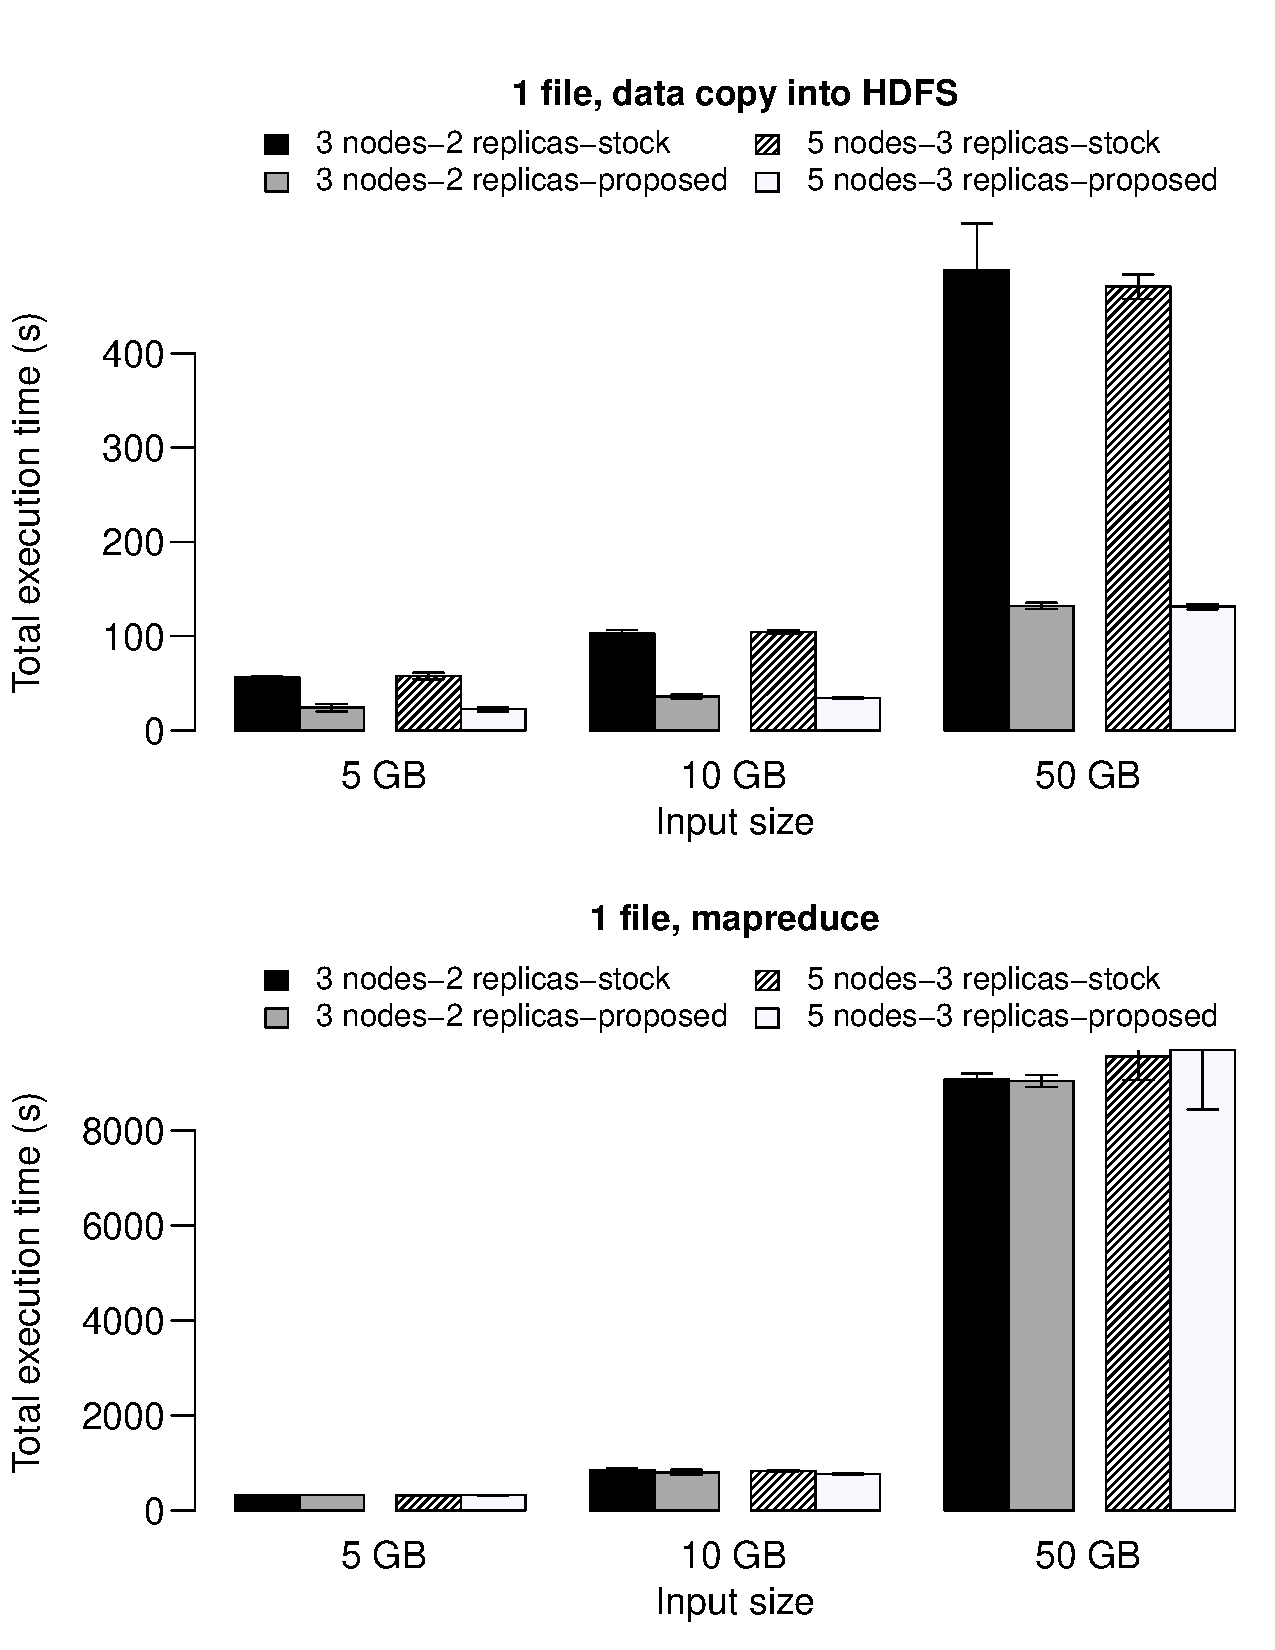
\includegraphics[width=\columnwidth, keepaspectratio]{result4.pdf}
\caption{Evaluation results for~\textit{TeraSort}}
\label{terasortres}
\end{figure}

The upper sub-plot of Figure~\ref{terasortres} shows that data copy times increase as the input
size is increased from 5 GB to 50 GB for both stock and proposed Hadoop. This is expected for stock
Hadoop; but, for our implementation, data copy times increase because records created by
the~\textit{TeraGen} are still processed one-by-one.~\textit{TeraGen} generates data in the format
of 100-byte records (i.e. to generate 6553600 bytes of data, 65536 records are needed) and it writes
data to each record individually. In the implementation presented in this work, these records
are created; but, actual data is not committed to HDFS resulting in empty records. As the input
size is increased from 5 GB to 50 GB, the number of records to create increases as well, which
in turn increases data copy time. Still, a data copy performance improvement by up to 73\% is
observed, which becomes even bigger with larger input sizes. Additionally, the number of replicas
and storage nodes does not affect the data copy performance significantly. For the MapReduce phase,
nearly 5\% improvement is observed due to data-compute locality, with the number of replicas or
storage nodes having no significant effect. MapReduce performance improvements in this
test case are not as high as those from~\textit{TestDFSIO}, as the MapReduce phase is not dominated by reads
only.

\section{Conclusions}
\label{conclusions}
In this paper, we presented an approach that performs computation
on existing large-scale data in an object storage system without moving
data anywhere and analyzed the outcomes of this approach. Experimental
evaluations with Hadoop and Ceph object-based storage system show that
it is possible to implement Hadoop on top of Ceph as a lightweight computational
framework and to perform computational tasks in-place alleviating the need to transfer
large-scale data to a remote compute cluster. Initial data copy
performance is improved by up to 96\% and MapReduce performance is
improved by up to 20\%.

Future research directions include implementing checksum calculation algorithms,
tests with more data and larger storage systems and making datanode block scans
work with symbolic links. The proposed approach in this paper
does not read any data into HDFS and performing checksum calculations without
reading any data into HDFS is tricky; because, Hadoop and the underlying storage
system might have different checksum calculation algorithms. As an example;
Hadoop uses CRC32; but, if the underlying storage system uses another checksum
algorithm (i.e. MD5), this at least requires converting one checksum calculation
method to another, which is a very expensive operation, even if no data is read
into HDFS. Additionally, performance evaluation tests in this work are conducted
with five nodes with three replicas at most. Further tests with different number
of nodes and replicas would be helpful to prove the effectiveness of our approach.
Finally, datanode block scans are disabled as they are detecting and invalidating
the symbolic links created in the proposed approach. They can be changed to resume their
normal functionality while not invalidating symbolic links; instead of disabling
them all together.
\label{sec-conclusion}

\section{Acknowledgement}
This work was supported in part by a NSF High End Computing University
Research Activity grant (award number CCF-0937879). Any opinions,
findings and conclusions or recommendations expressed in this material
are those of the authors and do not necessarily reflect those of the
NSF.

%% The Appendices part is started with the command \appendix;
%% appendix  are then done as normal 
%% \appendix

%% \section{}
%% \label{}

%% If you have bibdatabase file and want bibtex to generate the
%% bibitems, please use
%%
%\bibliographystyle{elsarticle-num} 
%\bibliography{jss}

%% else use the following coding to input the bibitems directly in the
%% TeX file.

%%\begin{thebibliography}{00}

%% \bibitem{label}
%% Text of bibliographic item

%%\bibitem{}

%%\end{thebibliography}
\begin{thebibliography}{10}
\expandafter\ifx\csname url\endcsname\relax
  \def\url#1{\texttt{#1}}\fi
\expandafter\ifx\csname urlprefix\endcsname\relax\def\urlprefix{URL }\fi
\expandafter\ifx\csname href\endcsname\relax
  \def\href#1#2{#2} \def\path#1{#1}\fi

\bibitem{amazon_ec2}
{Amazon Elastic Compute Cloud}, \url{http://aws.amazon.com/ec2/}.

\bibitem{idcbigdata}
J.~Gantz, D.~Reinsel, {The Digital Universe in 2020: Big Data, Bigger Digital
  Shadows, Biggest Growth in the Far East}, IDC iView: IDC Analyze the Future
  (2012) 1--16.

\bibitem{Gibson:1998:CHS:291006.291029}
G.~A. Gibson, D.~F. Nagle, K.~Amiri, J.~Butler, F.~W. Chang, H.~Gobioff,
  C.~Hardin, E.~Riedel, D.~Rochberg, J.~Zelenka,
  \href{http://doi.acm.org/10.1145/291006.291029}{A cost-effective,
  high-bandwidth storage architecture}, SIGPLAN Not. 33~(11) (1998) 92--103.
\newblock \href {http://dx.doi.org/10.1145/291006.291029}
  {\path{doi:10.1145/291006.291029}}.
\newline\urlprefix\url{http://doi.acm.org/10.1145/291006.291029}

\bibitem{1222722}
M.~Mesnier, G.~R. Ganger, E.~Riedel, Object-based storage, IEEE Communications
  Magazine 41~(8) (2003) 84--90.
\newblock \href {http://dx.doi.org/10.1109/MCOM.2003.1222722}
  {\path{doi:10.1109/MCOM.2003.1222722}}.

\bibitem{lustre_web}
{Lustre}, \url{http://wiki.lustre.org/index.php/Main\_Page}.

\bibitem{maltzahn2010ceph}
C.~Maltzahn, E.~Molina-Estolano, A.~Khurana, A.~J. Nelson, S.~A. Brandt,
  S.~Weil, {Ceph as a Scalable Alternative to the Hadoop Distributed File
  System}, {;login::The USENIX Magazine} 35~(4) (2010) 38--49.

\bibitem{openstack_swift}
{Swift}: Openstack object storage, \url{https://wiki.openstack.org/wiki/Swift}
  (2015).

\bibitem{revisitmd}
N.~Ali, A.~Devulapalli, D.~Dalessandro, P.~Wyckoff, P.~Sadayappan, Revisiting
  the metadata architecture of parallel file systems, in: Petascale Data
  Storage Workshop, 2008. PDSW '08. 3rd, 2008, pp. 1--9.
\newblock \href {http://dx.doi.org/10.1109/PDSW.2008.4811892}
  {\path{doi:10.1109/PDSW.2008.4811892}}.

\bibitem{apache_hadoop}
K.~Shvachko, H.~Kuang, S.~Radia, R.~Chansler, The hadoop distributed file
  system, in: Mass Storage Systems and Technologies (MSST), 2010 IEEE 26th
  Symposium on, 2010, pp. 1--10.
\newblock \href {http://dx.doi.org/10.1109/MSST.2010.5496972}
  {\path{doi:10.1109/MSST.2010.5496972}}.

\bibitem{cephorig}
S.~A. Weil, S.~A. Brandt, E.~L. Miller, D.~D.~E. Long, C.~Maltzahn,
  \href{http://dl.acm.org/citation.cfm?id=1298455.1298485}{Ceph: A scalable,
  high-performance distributed file system}, in: Proceedings of the 7th
  Symposium on Operating Systems Design and Implementation, OSDI '06, USENIX
  Association, Berkeley, CA, USA, 2006, pp. 307--320.
\newline\urlprefix\url{http://dl.acm.org/citation.cfm?id=1298455.1298485}

\bibitem{hadoopgrep}
{Hadoop Grep}, \url{https://wiki.apache.org/hadoop/Grep}.

\bibitem{hadoopwordcount}
{Hadoop WordCount}, \url{https://wiki.apache.org/hadoop/WordCount}.

\bibitem{hadooptestdfsio}
{Benchmarking and Stress Testing an Hadoop Cluster with TeraSort, TestDFSIO \&
  Co.},
  \url{http://www.michael-noll.com/blog/2011/04/09/benchmarking-and-stress-testing-an-hadoop-cluster-with-terasort-testdfsio-nnbench-mrbench/}.

\bibitem{hadoopterasort}
{Hadoop TeraSort},
  \url{https://hadoop.apache.org/docs/r1.2.1/api/org/apache/hadoop/examples/terasort/package-summary.html}.

\bibitem{Dean:2008:MSD:1327452.1327492}
J.~Dean, S.~Ghemawat,
  \href{http://doi.acm.org/10.1145/1327452.1327492}{Mapreduce: Simplified data
  processing on large clusters}, Commun. ACM 51~(1) (2008) 107--113.
\newblock \href {http://dx.doi.org/10.1145/1327452.1327492}
  {\path{doi:10.1145/1327452.1327492}}.
\newline\urlprefix\url{http://doi.acm.org/10.1145/1327452.1327492}

\bibitem{osd3}
{T10 Technical Committee of the InterNational Committee on Information
  Technology Standards}, Object-{Based} {Storage} {Devices} - 3 {(OSD-3)},
  \url{http://www.t10.org/}.

\bibitem{Carns:2000:PPF:1268379.1268407}
P.~H. Carns, W.~B. Ligon, III, R.~B. Ross, R.~Thakur,
  \href{http://dl.acm.org/citation.cfm?id=1268379.1268407}{Pvfs: A parallel
  file system for linux clusters}, in: Proceedings of the 4th Annual Linux
  Showcase \& Conference - Volume 4, ALS'00, USENIX Association, Berkeley, CA,
  USA, 2000, pp. 28--28.
\newline\urlprefix\url{http://dl.acm.org/citation.cfm?id=1268379.1268407}

\bibitem{amazon_s3}
{Amazon Simple Storage Service}, \url{http://aws.amazon.com/s3/}.

\bibitem{shvachko2010hdfs}
K.~V. Shvachko, {HDFS Scalability: The Limits to Growth}, ;login::The USENIX
  Magazine 35~(2) (2010) 6--16.

\bibitem{Ananthanarayanan:2011:SCS:1966445.1966472}
G.~Ananthanarayanan, S.~Agarwal, S.~Kandula, A.~Greenberg, I.~Stoica,
  D.~Harlan, E.~Harris,
  \href{http://doi.acm.org/10.1145/1966445.1966472}{Scarlett: Coping with
  skewed content popularity in mapreduce clusters}, in: Proceedings of the
  Sixth Conference on Computer Systems, EuroSys '11, ACM, New York, NY, USA,
  2011, pp. 287--300.
\newblock \href {http://dx.doi.org/10.1145/1966445.1966472}
  {\path{doi:10.1145/1966445.1966472}}.
\newline\urlprefix\url{http://doi.acm.org/10.1145/1966445.1966472}

\bibitem{Porter:2010:DSC:1773912.1773923}
G.~Porter, \href{http://doi.acm.org/10.1145/1773912.1773923}{Decoupling storage
  and computation in hadoop with superdatanodes}, SIGOPS Oper. Syst. Rev.
  44~(2) (2010) 41--46.
\newblock \href {http://dx.doi.org/10.1145/1773912.1773923}
  {\path{doi:10.1145/1773912.1773923}}.
\newline\urlprefix\url{http://doi.acm.org/10.1145/1773912.1773923}

\bibitem{Eltabakh:2011:CFD:2002938.2002943}
M.~Y. Eltabakh, Y.~Tian, F.~\"{O}zcan, R.~Gemulla, A.~Krettek, J.~McPherson,
  \href{http://dx.doi.org/10.14778/2002938.2002943}{Cohadoop: Flexible data
  placement and its exploitation in hadoop}, Proc. VLDB Endow. 4~(9) (2011)
  575--585.
\newblock \href {http://dx.doi.org/10.14778/2002938.2002943}
  {\path{doi:10.14778/2002938.2002943}}.
\newline\urlprefix\url{http://dx.doi.org/10.14778/2002938.2002943}

\bibitem{6217451}
S.~Ibrahim, H.~Jin, L.~Lu, B.~He, G.~Antoniu, S.~Wu, Maestro: Replica-aware map
  scheduling for mapreduce, in: Cluster, Cloud and Grid Computing (CCGrid),
  2012 12th IEEE/ACM International Symposium on, 2012, pp. 435--442.
\newblock \href {http://dx.doi.org/10.1109/CCGrid.2012.122}
  {\path{doi:10.1109/CCGrid.2012.122}}.

\bibitem{Tantisiriroj:2011:DDF:2063384.2063474}
W.~Tantisiriroj, S.~W. Son, S.~Patil, S.~J. Lang, G.~Gibson, R.~B. Ross,
  \href{http://doi.acm.org/10.1145/2063384.2063474}{On the duality of
  data-intensive file system design: Reconciling hdfs and pvfs}, in:
  Proceedings of 2011 International Conference for High Performance Computing,
  Networking, Storage and Analysis, SC '11, ACM, New York, NY, USA, 2011, pp.
  67:1--67:12.
\newblock \href {http://dx.doi.org/10.1145/2063384.2063474}
  {\path{doi:10.1145/2063384.2063474}}.
\newline\urlprefix\url{http://doi.acm.org/10.1145/2063384.2063474}

\bibitem{Ananthanarayanan:2009:CAW:1855533.1855548}
R.~Ananthanarayanan, K.~Gupta, P.~Pandey, H.~Pucha, P.~Sarkar, M.~Shah,
  R.~Tewari, \href{http://dl.acm.org/citation.cfm?id=1855533.1855548}{Cloud
  analytics: Do we really need to reinvent the storage stack?}, in: Proceedings
  of the 2009 Conference on Hot Topics in Cloud Computing, HotCloud'09, USENIX
  Association, Berkeley, CA, USA, 2009.
\newline\urlprefix\url{http://dl.acm.org/citation.cfm?id=1855533.1855548}

\bibitem{lustre_with_hadoop}
{Using Lustre with Apache Hadoop, Sun Microsystems Inc.},
  \url{http://wiki.lustre.org/images/1/1b/Hadoop\_wp\_v0.4.2.pdf}.

\bibitem{rupprechtbd}
L.~Rupprecht, R.~Zhang, D.~Hildebrand, {Big Data Analytics on Object Stores: A
  Performance Study}, in: SC14: International Conference for High Performance
  Computing, Networking, Storage and Analysis, New Orleans, LA, USA, 2014.

\bibitem{chengcast}
Y.~Cheng, M.~S. Iqbal, A.~Gupta, A.~R. Butt,
  \href{http://doi.acm.org/10.1145/2749246.2749252}{Cast: Tiering storage for
  data analytics in the cloud}, in: Proceedings of the 24th International
  Symposium on High-Performance Parallel and Distributed Computing, HPDC '15,
  ACM, New York, NY, USA, 2015, pp. 45--56.
\newblock \href {http://dx.doi.org/10.1145/2749246.2749252}
  {\path{doi:10.1145/2749246.2749252}}.
\newline\urlprefix\url{http://doi.acm.org/10.1145/2749246.2749252}

\bibitem{supmr}
M.~Sevilla, I.~Nassi, K.~Ioannidou, S.~Brandt, C.~Maltzahn, Supmr:
  Circumventing disk and memory bandwidth bottlenecks for scale-up mapreduce,
  in: Parallel Distributed Processing Symposium Workshops (IPDPSW), 2014 IEEE
  International, 2014, pp. 1505--1514.
\newblock \href {http://dx.doi.org/10.1109/IPDPSW.2014.168}
  {\path{doi:10.1109/IPDPSW.2014.168}}.

\bibitem{nakshatra}
A.~Kathpal, G.~Yasa, Nakshatra: Towards running batch analytics on an archive,
  in: Modelling, Analysis Simulation of Computer and Telecommunication Systems
  (MASCOTS), 2014 IEEE 22nd International Symposium on, 2014, pp. 479--482.
\newblock \href {http://dx.doi.org/10.1109/MASCOTS.2014.67}
  {\path{doi:10.1109/MASCOTS.2014.67}}.

\bibitem{vncache}
B.~Palanisamy, A.~Singh, N.~Mandagere, G.~Alatorre, L.~Liu, Mapreduce analysis
  for cloud-archived data, 2014 14th IEEE/ACM International Symposium on
  Cluster, Cloud and Grid Computing 0 (2014) 51--60.
\newblock \href
  {http://dx.doi.org/http://doi.ieeecomputersociety.org/10.1109/CCGrid.2014.13}
  {\path{doi:http://doi.ieeecomputersociety.org/10.1109/CCGrid.2014.13}}.

\bibitem{180733}
M.~Mihailescu, G.~Soundararajan, C.~Amza,
  \href{http://dl.acm.org/citation.cfm?id=2342806.2342808}{Mixapart: Decoupled
  analytics for shared storage systems}, in: Proceedings of the 4th USENIX
  Conference on Hot Topics in Storage and File Systems, HotStorage'12, USENIX
  Association, Berkeley, CA, USA, 2012, pp. 2--2.
\newline\urlprefix\url{http://dl.acm.org/citation.cfm?id=2342806.2342808}

\bibitem{rutman}
N.~Rutman, {Map/Reduce on Lustre (white paper). Technical report.}, Xyratex
  Technology Limited, Havant, UK, 2011.

\bibitem{hadoopyarnprogress}
W.~Yu, O.~Kulkarni, {Progress Report on Efficient Integration of Lustre and
  Hadoop/YARN}, The Lustre User Group Conference, Miami, FL, USA, 2014.

\bibitem{hadooplustre}
C.~Xu, R.~Goldstone, Z.~Liu, H.~Chen, B.~Neitzel, W.~Yu, Exploiting analytics
  shipping with virtualized mapreduce on hpc backend storage servers, Parallel
  and Distributed Systems, IEEE Transactions on PP~(99) (2015) 1--1.
\newblock \href {http://dx.doi.org/10.1109/TPDS.2015.2389262}
  {\path{doi:10.1109/TPDS.2015.2389262}}.

\bibitem{wilsonhadoop}
E.~Wilson, M.~Kandemir, G.~Gibson, Will they blend?: Exploring big data
  computation atop traditional hpc nas storage, in: Distributed Computing
  Systems (ICDCS), 2014 IEEE 34th International Conference on, 2014, pp.
  524--534.
\newblock \href {http://dx.doi.org/10.1109/ICDCS.2014.60}
  {\path{doi:10.1109/ICDCS.2014.60}}.

\bibitem{gce}
{Google Cloud Platform - Compute Engine},
  \url{https://cloud.google.com/compute/}.

\bibitem{hadoopconf}
{Hadoop Cluster Setup},
  \url{http://hadoop.apache.org/docs/r1.2.1/cluster\_setup.html}.

\bibitem{hdfs941}
{Hadoop JIRA HDFS-941}, \url{https://issues.apache.org/jira/browse/HDFS-941}.

\end{thebibliography}
\end{document}
\endinput
%%
%% End of file `elsarticle-template-num.tex'.
